\documentclass[twoside]{book}

% Packages required by doxygen
\usepackage{calc}
\usepackage{doxygen}
\usepackage{graphicx}
\usepackage[utf8]{inputenc}
\usepackage{makeidx}
\usepackage{multicol}
\usepackage{multirow}
\usepackage{textcomp}
\usepackage[table]{xcolor}

% Font selection
\usepackage[T1]{fontenc}
\usepackage{mathptmx}
\usepackage[scaled=.90]{helvet}
\usepackage{courier}
\usepackage{amssymb}
\usepackage{sectsty}
\renewcommand{\familydefault}{\sfdefault}
\allsectionsfont{%
  \fontseries{bc}\selectfont%
  \color{darkgray}%
}
\renewcommand{\DoxyLabelFont}{%
  \fontseries{bc}\selectfont%
  \color{darkgray}%
}

% Page & text layout
\usepackage{geometry}
\geometry{%
  a4paper,%
  top=2.5cm,%
  bottom=2.5cm,%
  left=2.5cm,%
  right=2.5cm%
}
\tolerance=750
\hfuzz=15pt
\hbadness=750
\setlength{\emergencystretch}{15pt}
\setlength{\parindent}{0cm}
\setlength{\parskip}{0.2cm}
\makeatletter
\renewcommand{\paragraph}{%
  \@startsection{paragraph}{4}{0ex}{-1.0ex}{1.0ex}{%
    \normalfont\normalsize\bfseries\SS@parafont%
  }%
}
\renewcommand{\subparagraph}{%
  \@startsection{subparagraph}{5}{0ex}{-1.0ex}{1.0ex}{%
    \normalfont\normalsize\bfseries\SS@subparafont%
  }%
}
\makeatother

% Headers & footers
\usepackage{fancyhdr}
\pagestyle{fancyplain}
\fancyhead[LE]{\fancyplain{}{\bfseries\thepage}}
\fancyhead[CE]{\fancyplain{}{}}
\fancyhead[RE]{\fancyplain{}{\bfseries\leftmark}}
\fancyhead[LO]{\fancyplain{}{\bfseries\rightmark}}
\fancyhead[CO]{\fancyplain{}{}}
\fancyhead[RO]{\fancyplain{}{\bfseries\thepage}}
\fancyfoot[LE]{\fancyplain{}{}}
\fancyfoot[CE]{\fancyplain{}{}}
\fancyfoot[RE]{\fancyplain{}{\bfseries\scriptsize Generated on Mon Oct 7 2013 14:57:29 for SpeedGames by Doxygen }}
\fancyfoot[LO]{\fancyplain{}{\bfseries\scriptsize Generated on Mon Oct 7 2013 14:57:29 for SpeedGames by Doxygen }}
\fancyfoot[CO]{\fancyplain{}{}}
\fancyfoot[RO]{\fancyplain{}{}}
\renewcommand{\footrulewidth}{0.4pt}
\renewcommand{\chaptermark}[1]{%
  \markboth{#1}{}%
}
\renewcommand{\sectionmark}[1]{%
  \markright{\thesection\ #1}%
}

% Indices & bibliography
\usepackage{natbib}
\usepackage[titles]{tocloft}
\setcounter{tocdepth}{3}
\setcounter{secnumdepth}{5}
\makeindex

% Hyperlinks (required, but should be loaded last)
\usepackage{ifpdf}
\ifpdf
  \usepackage[pdftex,pagebackref=true]{hyperref}
\else
  \usepackage[ps2pdf,pagebackref=true]{hyperref}
\fi
\hypersetup{%
  colorlinks=true,%
  linkcolor=blue,%
  citecolor=blue,%
  unicode%
}

% Custom commands
\newcommand{\clearemptydoublepage}{%
  \newpage{\pagestyle{empty}\cleardoublepage}%
}


%===== C O N T E N T S =====

\begin{document}

% Titlepage & ToC
\hypersetup{pageanchor=false}
\pagenumbering{roman}
\begin{titlepage}
\vspace*{7cm}
\begin{center}%
{\Large Speed\-Games \\[1ex]\large 0.\-1 }\\
\vspace*{1cm}
{\large Generated by Doxygen 1.8.4}\\
\vspace*{0.5cm}
{\small Mon Oct 7 2013 14:57:29}\\
\end{center}
\end{titlepage}
\clearemptydoublepage
\tableofcontents
\clearemptydoublepage
\pagenumbering{arabic}
\hypersetup{pageanchor=true}

%--- Begin generated contents ---
\chapter{Class Index}
\section{Class List}
Here are the classes, structs, unions and interfaces with brief descriptions\-:\begin{DoxyCompactList}
\item\contentsline{section}{\hyperlink{classCard}{Card} }{\pageref{classCard}}{}
\item\contentsline{section}{\hyperlink{classCompany}{Company} }{\pageref{classCompany}}{}
\item\contentsline{section}{\hyperlink{classGame}{Game} }{\pageref{classGame}}{}
\item\contentsline{section}{\hyperlink{classMainScreen}{Main\-Screen} }{\pageref{classMainScreen}}{}
\item\contentsline{section}{\hyperlink{classPlayer}{Player} }{\pageref{classPlayer}}{}
\item\contentsline{section}{\hyperlink{classQuestion}{Question} }{\pageref{classQuestion}}{}
\end{DoxyCompactList}

\chapter{File Index}
\section{File List}
Here is a list of all files with brief descriptions\-:\begin{DoxyCompactList}
\item\contentsline{section}{\hyperlink{main_8cc}{main.\-cc} }{\pageref{main_8cc}}{}
\item\contentsline{section}{Card/\hyperlink{Card_8cc}{Card.\-cc} }{\pageref{Card_8cc}}{}
\item\contentsline{section}{Card/\hyperlink{Card_8h}{Card.\-h} }{\pageref{Card_8h}}{}
\item\contentsline{section}{Company/\hyperlink{Company_8cc}{Company.\-cc} }{\pageref{Company_8cc}}{}
\item\contentsline{section}{Company/\hyperlink{Company_8h}{Company.\-h} }{\pageref{Company_8h}}{}
\item\contentsline{section}{Game/\hyperlink{Game_8cc}{Game.\-cc} }{\pageref{Game_8cc}}{}
\item\contentsline{section}{Game/\hyperlink{Game_8h}{Game.\-h} }{\pageref{Game_8h}}{}
\item\contentsline{section}{Player/\hyperlink{Player_8cc}{Player.\-cc} }{\pageref{Player_8cc}}{}
\item\contentsline{section}{Player/\hyperlink{Player_8h}{Player.\-h} }{\pageref{Player_8h}}{}
\item\contentsline{section}{Question/\hyperlink{Question_8cc}{Question.\-cc} }{\pageref{Question_8cc}}{}
\item\contentsline{section}{Question/\hyperlink{Question_8h}{Question.\-h} }{\pageref{Question_8h}}{}
\item\contentsline{section}{Screen/\hyperlink{MainScreen_8cc}{Main\-Screen.\-cc} }{\pageref{MainScreen_8cc}}{}
\item\contentsline{section}{Screen/\hyperlink{MainScreen_8h}{Main\-Screen.\-h} }{\pageref{MainScreen_8h}}{}
\end{DoxyCompactList}

\chapter{Class Documentation}
\hypertarget{classCard}{\section{Card Class Reference}
\label{classCard}\index{Card@{Card}}
}


{\ttfamily \#include $<$Card.\-h$>$}

\subsection*{Public Member Functions}
\begin{DoxyCompactItemize}
\item 
\hyperlink{classCard_a849a1503562f1c3bc80134d4eab83d99}{Card} (const char $\ast$image, int effect, int magnitude, int id)
\item 
int \hyperlink{classCard_a7cc686dc64c240cf346d6a676b9fa57d}{get\-Effect} ()
\item 
int \hyperlink{classCard_a03bec0d54ee5c50e76d690b9ca73954b}{get\-Magnitude} ()
\item 
int \hyperlink{classCard_a017122109ae10b3c0cce6b267f323414}{get\-Id} ()
\end{DoxyCompactItemize}


\subsection{Constructor \& Destructor Documentation}
\hypertarget{classCard_a849a1503562f1c3bc80134d4eab83d99}{\index{Card@{Card}!Card@{Card}}
\index{Card@{Card}!Card@{Card}}
\subsubsection[{Card}]{\setlength{\rightskip}{0pt plus 5cm}Card\-::\-Card (
\begin{DoxyParamCaption}
\item[{const char $\ast$}]{image, }
\item[{int}]{effect, }
\item[{int}]{magnitude, }
\item[{int}]{id}
\end{DoxyParamCaption}
)}}\label{classCard_a849a1503562f1c3bc80134d4eab83d99}


\subsection{Member Function Documentation}
\hypertarget{classCard_a7cc686dc64c240cf346d6a676b9fa57d}{\index{Card@{Card}!get\-Effect@{get\-Effect}}
\index{get\-Effect@{get\-Effect}!Card@{Card}}
\subsubsection[{get\-Effect}]{\setlength{\rightskip}{0pt plus 5cm}int Card\-::get\-Effect (
\begin{DoxyParamCaption}
{}
\end{DoxyParamCaption}
)}}\label{classCard_a7cc686dc64c240cf346d6a676b9fa57d}
\hypertarget{classCard_a017122109ae10b3c0cce6b267f323414}{\index{Card@{Card}!get\-Id@{get\-Id}}
\index{get\-Id@{get\-Id}!Card@{Card}}
\subsubsection[{get\-Id}]{\setlength{\rightskip}{0pt plus 5cm}int Card\-::get\-Id (
\begin{DoxyParamCaption}
{}
\end{DoxyParamCaption}
)}}\label{classCard_a017122109ae10b3c0cce6b267f323414}
\hypertarget{classCard_a03bec0d54ee5c50e76d690b9ca73954b}{\index{Card@{Card}!get\-Magnitude@{get\-Magnitude}}
\index{get\-Magnitude@{get\-Magnitude}!Card@{Card}}
\subsubsection[{get\-Magnitude}]{\setlength{\rightskip}{0pt plus 5cm}int Card\-::get\-Magnitude (
\begin{DoxyParamCaption}
{}
\end{DoxyParamCaption}
)}}\label{classCard_a03bec0d54ee5c50e76d690b9ca73954b}


The documentation for this class was generated from the following file\-:\begin{DoxyCompactItemize}
\item 
Card/\hyperlink{Card_8h}{Card.\-h}\end{DoxyCompactItemize}

\hypertarget{classCompany}{\section{Company Class Reference}
\label{classCompany}\index{Company@{Company}}
}


{\ttfamily \#include $<$Company.\-h$>$}

\subsection*{Public Member Functions}
\begin{DoxyCompactItemize}
\item 
\hyperlink{classCompany_a3487b164500da1693c1ff028b55a4511}{Company} (const char $\ast$name)
\item 
const char $\ast$ \hyperlink{classCompany_a368dd41a62752e49b4b43052548920ab}{get\-Name} () const 
\item 
void \hyperlink{classCompany_ad38560ac7e495830ed55568a0f4f3321}{up\-Level} ()
\item 
void \hyperlink{classCompany_adf93037d4dd38136f5921afcde718ce6}{down\-Level} ()
\item 
int \hyperlink{classCompany_a724de8d3a259952e4b434eaa51d1564d}{get\-Level} () const 
\item 
int \hyperlink{classCompany_aa66f315e9f43f7818457ca424106e322}{get\-Certification\-Cost} () const 
\end{DoxyCompactItemize}


\subsection{Constructor \& Destructor Documentation}
\hypertarget{classCompany_a3487b164500da1693c1ff028b55a4511}{\index{Company@{Company}!Company@{Company}}
\index{Company@{Company}!Company@{Company}}
\subsubsection[{Company}]{\setlength{\rightskip}{0pt plus 5cm}Company\-::\-Company (
\begin{DoxyParamCaption}
\item[{const char $\ast$}]{name}
\end{DoxyParamCaption}
)}}\label{classCompany_a3487b164500da1693c1ff028b55a4511}

\begin{DoxyCode}
7 \{
8     nameCompany = name;
9     levelCMMI = 1;
10 \}
\end{DoxyCode}


\subsection{Member Function Documentation}
\hypertarget{classCompany_adf93037d4dd38136f5921afcde718ce6}{\index{Company@{Company}!down\-Level@{down\-Level}}
\index{down\-Level@{down\-Level}!Company@{Company}}
\subsubsection[{down\-Level}]{\setlength{\rightskip}{0pt plus 5cm}void Company\-::down\-Level (
\begin{DoxyParamCaption}
{}
\end{DoxyParamCaption}
)}}\label{classCompany_adf93037d4dd38136f5921afcde718ce6}

\begin{DoxyCode}
19 \{
20     \textcolor{keywordflow}{if} (levelCMMI > 1)
21         levelCMMI -= 1;
22 \}
\end{DoxyCode}
\hypertarget{classCompany_aa66f315e9f43f7818457ca424106e322}{\index{Company@{Company}!get\-Certification\-Cost@{get\-Certification\-Cost}}
\index{get\-Certification\-Cost@{get\-Certification\-Cost}!Company@{Company}}
\subsubsection[{get\-Certification\-Cost}]{\setlength{\rightskip}{0pt plus 5cm}int Company\-::get\-Certification\-Cost (
\begin{DoxyParamCaption}
{}
\end{DoxyParamCaption}
) const}}\label{classCompany_aa66f315e9f43f7818457ca424106e322}

\begin{DoxyCode}
25 \{
26     \textcolor{comment}{//TODO}
27 
28     \textcolor{keywordflow}{return} 100000 * levelCMMI;
29 \}
\end{DoxyCode}
\hypertarget{classCompany_a724de8d3a259952e4b434eaa51d1564d}{\index{Company@{Company}!get\-Level@{get\-Level}}
\index{get\-Level@{get\-Level}!Company@{Company}}
\subsubsection[{get\-Level}]{\setlength{\rightskip}{0pt plus 5cm}int Company\-::get\-Level (
\begin{DoxyParamCaption}
{}
\end{DoxyParamCaption}
) const\hspace{0.3cm}{\ttfamily [inline]}}}\label{classCompany_a724de8d3a259952e4b434eaa51d1564d}

\begin{DoxyCode}
17 \{ \textcolor{keywordflow}{return} levelCMMI; \}
\end{DoxyCode}
\hypertarget{classCompany_a368dd41a62752e49b4b43052548920ab}{\index{Company@{Company}!get\-Name@{get\-Name}}
\index{get\-Name@{get\-Name}!Company@{Company}}
\subsubsection[{get\-Name}]{\setlength{\rightskip}{0pt plus 5cm}const char$\ast$ Company\-::get\-Name (
\begin{DoxyParamCaption}
{}
\end{DoxyParamCaption}
) const\hspace{0.3cm}{\ttfamily [inline]}}}\label{classCompany_a368dd41a62752e49b4b43052548920ab}

\begin{DoxyCode}
13 \{ \textcolor{keywordflow}{return} nameCompany.data(); \}
\end{DoxyCode}
\hypertarget{classCompany_ad38560ac7e495830ed55568a0f4f3321}{\index{Company@{Company}!up\-Level@{up\-Level}}
\index{up\-Level@{up\-Level}!Company@{Company}}
\subsubsection[{up\-Level}]{\setlength{\rightskip}{0pt plus 5cm}void Company\-::up\-Level (
\begin{DoxyParamCaption}
{}
\end{DoxyParamCaption}
)}}\label{classCompany_ad38560ac7e495830ed55568a0f4f3321}

\begin{DoxyCode}
13 \{
14     \textcolor{keywordflow}{if} (levelCMMI < 5)
15         levelCMMI += 1;
16 \}
\end{DoxyCode}


The documentation for this class was generated from the following files\-:\begin{DoxyCompactItemize}
\item 
Company/\hyperlink{Company_8h}{Company.\-h}\item 
Company/\hyperlink{Company_8cc}{Company.\-cc}\end{DoxyCompactItemize}

\hypertarget{classGame}{\section{Game Class Reference}
\label{classGame}\index{Game@{Game}}
}


{\ttfamily \#include $<$Game.\-h$>$}

\subsection*{Public Member Functions}
\begin{DoxyCompactItemize}
\item 
\hyperlink{classGame_a44f47382ce13570a98591a8248b65316}{Game} (const std\-::list$<$ std\-::pair$<$ std\-::pair$<$ const char $\ast$, const char $\ast$ $>$, const char $\ast$ $>$ $>$ \&info\-Players, int num\-Rounds)
\item 
void \hyperlink{classGame_ae8638ccdb0ef3bf39a6affa30aa1258f}{start\-Game} ()
\end{DoxyCompactItemize}


\subsection{Constructor \& Destructor Documentation}
\hypertarget{classGame_a44f47382ce13570a98591a8248b65316}{\index{Game@{Game}!Game@{Game}}
\index{Game@{Game}!Game@{Game}}
\subsubsection[{Game}]{\setlength{\rightskip}{0pt plus 5cm}Game\-::\-Game (
\begin{DoxyParamCaption}
\item[{const std\-::list$<$ std\-::pair$<$ std\-::pair$<$ const char $\ast$, const char $\ast$ $>$, const char $\ast$ $>$ $>$ \&}]{info\-Players, }
\item[{int}]{num\-Rounds}
\end{DoxyParamCaption}
)}}\label{classGame_a44f47382ce13570a98591a8248b65316}

\begin{DoxyCode}
8 \{
9     \textcolor{keywordflow}{for} (list< pair<pair<const char*, const char*>, \textcolor{keyword}{const} \textcolor{keywordtype}{char}*> >::const\_iterator it = infoPlayers.begin()
      ; it != infoPlayers.end(); ++it)
10     \{
11         \hyperlink{classPlayer}{Player} player(it->first.first, it->first.second, it->second);
12         players.push\_back(player);
13     \}
14 
15     numberRounds = numRounds;
16     currentRound = 1;
17 \}
\end{DoxyCode}


\subsection{Member Function Documentation}
\hypertarget{classGame_ae8638ccdb0ef3bf39a6affa30aa1258f}{\index{Game@{Game}!start\-Game@{start\-Game}}
\index{start\-Game@{start\-Game}!Game@{Game}}
\subsubsection[{start\-Game}]{\setlength{\rightskip}{0pt plus 5cm}void Game\-::start\-Game (
\begin{DoxyParamCaption}
{}
\end{DoxyParamCaption}
)}}\label{classGame_ae8638ccdb0ef3bf39a6affa30aa1258f}

\begin{DoxyCode}
20 \{
21     \hyperlink{classMainScreen}{MainScreen} screen;
22     \textcolor{keywordflow}{while} (currentRound <= numberRounds)
23     \{
24         round(screen);
25         currentRound++;
26     \}
27 
28     endGame();
29 \}
\end{DoxyCode}


The documentation for this class was generated from the following files\-:\begin{DoxyCompactItemize}
\item 
Game/\hyperlink{Game_8h}{Game.\-h}\item 
Game/\hyperlink{Game_8cc}{Game.\-cc}\end{DoxyCompactItemize}

\hypertarget{classMainScreen}{\section{Main\-Screen Class Reference}
\label{classMainScreen}\index{Main\-Screen@{Main\-Screen}}
}


{\ttfamily \#include $<$Main\-Screen.\-h$>$}

\subsection*{Public Member Functions}
\begin{DoxyCompactItemize}
\item 
\hyperlink{classMainScreen_afe04f97c6cbff7dc13f03344c74e3253}{Main\-Screen} ()
\item 
int \hyperlink{classMainScreen_aa060b16684e89d25104f2fa9cc751961}{draw\-Screen} (const char $\ast$file\-Image\-Avatar, int num\-Round, int max\-Rounds, const char $\ast$name\-Player, const char $\ast$methodology\-Player, int points, int resources, const std\-::list$<$ std\-::pair$<$ const char $\ast$, int $>$ $>$ \&companies\-Player, const std\-::list$<$ std\-::pair$<$ const char $\ast$, int $>$ $>$ \&other\-Players)
\item 
int \hyperlink{classMainScreen_a44cfe11e0495894b7cce6fbba1395a90}{wait\-For\-Event} ()
\item 
void \hyperlink{classMainScreen_a055b854813b4a149f4eb43d0a7a4c574}{show\-Message} (const char $\ast$caption, const char $\ast$header, const char $\ast$text, bool error)
\item 
\hyperlink{classMainScreen_afe04f97c6cbff7dc13f03344c74e3253}{Main\-Screen} ()
\item 
int \hyperlink{classMainScreen_aa060b16684e89d25104f2fa9cc751961}{draw\-Screen} (const char $\ast$file\-Image\-Avatar, int num\-Round, int max\-Rounds, const char $\ast$name\-Player, const char $\ast$methodology\-Player, int points, int resources, const std\-::list$<$ std\-::pair$<$ const char $\ast$, int $>$ $>$ \&companies\-Player, const std\-::list$<$ std\-::pair$<$ const char $\ast$, int $>$ $>$ \&other\-Players)
\item 
int \hyperlink{classMainScreen_a44cfe11e0495894b7cce6fbba1395a90}{wait\-For\-Event} ()
\item 
void \hyperlink{classMainScreen_a055b854813b4a149f4eb43d0a7a4c574}{show\-Message} (const char $\ast$caption, const char $\ast$header, const char $\ast$text, bool error)
\end{DoxyCompactItemize}


\subsection{Constructor \& Destructor Documentation}
\hypertarget{classMainScreen_afe04f97c6cbff7dc13f03344c74e3253}{\index{Main\-Screen@{Main\-Screen}!Main\-Screen@{Main\-Screen}}
\index{Main\-Screen@{Main\-Screen}!MainScreen@{Main\-Screen}}
\subsubsection[{Main\-Screen}]{\setlength{\rightskip}{0pt plus 5cm}Main\-Screen\-::\-Main\-Screen (
\begin{DoxyParamCaption}
{}
\end{DoxyParamCaption}
)}}\label{classMainScreen_afe04f97c6cbff7dc13f03344c74e3253}

\begin{DoxyCode}
13 \{
14     display = NULL;
15     imageRoullete = NULL;
16     angle = 0.0;
17     height = 0;
18     width = 0;
19 \}
\end{DoxyCode}
\hypertarget{classMainScreen_afe04f97c6cbff7dc13f03344c74e3253}{\index{Main\-Screen@{Main\-Screen}!Main\-Screen@{Main\-Screen}}
\index{Main\-Screen@{Main\-Screen}!MainScreen@{Main\-Screen}}
\subsubsection[{Main\-Screen}]{\setlength{\rightskip}{0pt plus 5cm}Main\-Screen\-::\-Main\-Screen (
\begin{DoxyParamCaption}
{}
\end{DoxyParamCaption}
)}}\label{classMainScreen_afe04f97c6cbff7dc13f03344c74e3253}


\subsection{Member Function Documentation}
\hypertarget{classMainScreen_aa060b16684e89d25104f2fa9cc751961}{\index{Main\-Screen@{Main\-Screen}!draw\-Screen@{draw\-Screen}}
\index{draw\-Screen@{draw\-Screen}!MainScreen@{Main\-Screen}}
\subsubsection[{draw\-Screen}]{\setlength{\rightskip}{0pt plus 5cm}int Main\-Screen\-::draw\-Screen (
\begin{DoxyParamCaption}
\item[{const char $\ast$}]{file\-Image\-Avatar, }
\item[{int}]{num\-Round, }
\item[{int}]{max\-Rounds, }
\item[{const char $\ast$}]{name\-Player, }
\item[{const char $\ast$}]{methodology\-Player, }
\item[{int}]{points, }
\item[{int}]{resources, }
\item[{const std\-::list$<$ std\-::pair$<$ const char $\ast$, int $>$ $>$ \&}]{companies\-Player, }
\item[{const std\-::list$<$ std\-::pair$<$ const char $\ast$, int $>$ $>$ \&}]{other\-Players}
\end{DoxyParamCaption}
)}}\label{classMainScreen_aa060b16684e89d25104f2fa9cc751961}
\hypertarget{classMainScreen_aa060b16684e89d25104f2fa9cc751961}{\index{Main\-Screen@{Main\-Screen}!draw\-Screen@{draw\-Screen}}
\index{draw\-Screen@{draw\-Screen}!MainScreen@{Main\-Screen}}
\subsubsection[{draw\-Screen}]{\setlength{\rightskip}{0pt plus 5cm}int Main\-Screen\-::draw\-Screen (
\begin{DoxyParamCaption}
\item[{const char $\ast$}]{file\-Image\-Avatar, }
\item[{int}]{num\-Round, }
\item[{int}]{max\-Rounds, }
\item[{const char $\ast$}]{name\-Player, }
\item[{const char $\ast$}]{methodology\-Player, }
\item[{int}]{points, }
\item[{int}]{resources, }
\item[{const std\-::list$<$ std\-::pair$<$ const char $\ast$, int $>$ $>$ \&}]{companies\-Player, }
\item[{const std\-::list$<$ std\-::pair$<$ const char $\ast$, int $>$ $>$ \&}]{other\-Players}
\end{DoxyParamCaption}
)}}\label{classMainScreen_aa060b16684e89d25104f2fa9cc751961}
\hypertarget{classMainScreen_a055b854813b4a149f4eb43d0a7a4c574}{\index{Main\-Screen@{Main\-Screen}!show\-Message@{show\-Message}}
\index{show\-Message@{show\-Message}!MainScreen@{Main\-Screen}}
\subsubsection[{show\-Message}]{\setlength{\rightskip}{0pt plus 5cm}void Main\-Screen\-::show\-Message (
\begin{DoxyParamCaption}
\item[{const char $\ast$}]{caption, }
\item[{const char $\ast$}]{header, }
\item[{const char $\ast$}]{text, }
\item[{bool}]{error}
\end{DoxyParamCaption}
)}}\label{classMainScreen_a055b854813b4a149f4eb43d0a7a4c574}
\hypertarget{classMainScreen_a055b854813b4a149f4eb43d0a7a4c574}{\index{Main\-Screen@{Main\-Screen}!show\-Message@{show\-Message}}
\index{show\-Message@{show\-Message}!MainScreen@{Main\-Screen}}
\subsubsection[{show\-Message}]{\setlength{\rightskip}{0pt plus 5cm}void Main\-Screen\-::show\-Message (
\begin{DoxyParamCaption}
\item[{const char $\ast$}]{caption, }
\item[{const char $\ast$}]{header, }
\item[{const char $\ast$}]{text, }
\item[{bool}]{error}
\end{DoxyParamCaption}
)}}\label{classMainScreen_a055b854813b4a149f4eb43d0a7a4c574}

\begin{DoxyCode}
189 \{
190     \textcolor{keywordflow}{if} (error)
191         al\_show\_native\_message\_box(display, caption, header, text, NULL, ALLEGRO\_MESSAGEBOX\_ERROR);
192     \textcolor{keywordflow}{else}
193         al\_show\_native\_message\_box(display, caption, header, text, \textcolor{stringliteral}{"OK"}, ALLEGRO\_MESSAGEBOX\_OK\_CANCEL);
194 \}
\end{DoxyCode}
\hypertarget{classMainScreen_a44cfe11e0495894b7cce6fbba1395a90}{\index{Main\-Screen@{Main\-Screen}!wait\-For\-Event@{wait\-For\-Event}}
\index{wait\-For\-Event@{wait\-For\-Event}!MainScreen@{Main\-Screen}}
\subsubsection[{wait\-For\-Event}]{\setlength{\rightskip}{0pt plus 5cm}int Main\-Screen\-::wait\-For\-Event (
\begin{DoxyParamCaption}
{}
\end{DoxyParamCaption}
)}}\label{classMainScreen_a44cfe11e0495894b7cce6fbba1395a90}
\hypertarget{classMainScreen_a44cfe11e0495894b7cce6fbba1395a90}{\index{Main\-Screen@{Main\-Screen}!wait\-For\-Event@{wait\-For\-Event}}
\index{wait\-For\-Event@{wait\-For\-Event}!MainScreen@{Main\-Screen}}
\subsubsection[{wait\-For\-Event}]{\setlength{\rightskip}{0pt plus 5cm}int Main\-Screen\-::wait\-For\-Event (
\begin{DoxyParamCaption}
{}
\end{DoxyParamCaption}
)}}\label{classMainScreen_a44cfe11e0495894b7cce6fbba1395a90}

\begin{DoxyCode}
149 \{
150     ALLEGRO\_EVENT\_QUEUE *queue = al\_create\_event\_queue();
151     ALLEGRO\_EVENT event;
152     al\_register\_event\_source(queue, al\_get\_mouse\_event\_source());
153 
154     \textcolor{keywordflow}{while} (1)
155     \{
156         al\_wait\_for\_event(queue, &event);
157         \textcolor{keywordflow}{if} (event.type == ALLEGRO\_EVENT\_MOUSE\_BUTTON\_DOWN)
158         \{
159             \textcolor{keywordtype}{int} centerX = \hyperlink{MainScreen_8h_a95248267b1e9860a49b38b91d6060ac3}{VERT\_LINE\_PLAYERS\_WIDTH} * width / 2;
160             \textcolor{keywordtype}{int} centerY = (\hyperlink{MainScreen_8h_a317b5109da7c376133ac189c84b42640}{HOR\_LINE\_INFO\_PLAYER\_HEIGHT} - 
      \hyperlink{MainScreen_8h_a7e18b3decda36fa1ea88693a2e3db612}{HOR\_LINE\_ROUNDS\_HEIGHT}) * height / 2;
161             \textcolor{keywordtype}{double} dist = (\textcolor{keyword}{event}.mouse.x - centerX) * (event.mouse.x - centerX) + (\textcolor{keyword}{event}.mouse.y - centerY)
       * (event.mouse.y - centerY);
162             \textcolor{keywordflow}{if} (dist <= 16900)
163                 \textcolor{keywordflow}{return} rotateRoullete();
164             \textcolor{keywordflow}{else} \textcolor{keywordflow}{if} (event.mouse.y < 215 && event.mouse.y > 135 && event.mouse.x < 
      \hyperlink{MainScreen_8h_a95248267b1e9860a49b38b91d6060ac3}{VERT\_LINE\_PLAYERS\_WIDTH} * width && 
165                 event.mouse.x > \hyperlink{MainScreen_8h_a95248267b1e9860a49b38b91d6060ac3}{VERT\_LINE\_PLAYERS\_WIDTH} * width - 200)
166             \{
167                 \textcolor{keywordflow}{if} (confirmPurchase() == 1)
168                     \textcolor{keywordflow}{return} 11;
169                 \textcolor{keywordflow}{else}
170                     \textcolor{keywordflow}{return} 0;
171             \}
172             \textcolor{keywordflow}{else} \textcolor{keywordflow}{if} (event.mouse.y < 315 && event.mouse.y > 235 && event.mouse.x < 
      \hyperlink{MainScreen_8h_a95248267b1e9860a49b38b91d6060ac3}{VERT\_LINE\_PLAYERS\_WIDTH} * width && 
173                 event.mouse.x > \hyperlink{MainScreen_8h_a95248267b1e9860a49b38b91d6060ac3}{VERT\_LINE\_PLAYERS\_WIDTH} * width - 200)
174             \{
175                 \textcolor{keywordtype}{int} answer = confirmCertification();
176                 \textcolor{keywordflow}{if} (answer == 0)
177                     \textcolor{keywordflow}{return} 0;
178                 \textcolor{keywordflow}{else}
179                     \textcolor{keywordflow}{return} 11 + answer;
180             \}
181         \}
182     \}
183 
184     \textcolor{keywordflow}{return} 0;
185 \}
\end{DoxyCode}


The documentation for this class was generated from the following files\-:\begin{DoxyCompactItemize}
\item 
Screen/\hyperlink{MainScreen_8h}{Main\-Screen.\-h}\item 
Screen/\hyperlink{Screen_8h}{Screen.\-h}\item 
Screen/\hyperlink{MainScreen_8cc}{Main\-Screen.\-cc}\item 
Screen/\hyperlink{Screen_8cc}{Screen.\-cc}\end{DoxyCompactItemize}

\hypertarget{classPlayer}{\section{Player Class Reference}
\label{classPlayer}\index{Player@{Player}}
}


{\ttfamily \#include $<$Player.\-h$>$}

\subsection*{Public Member Functions}
\begin{DoxyCompactItemize}
\item 
\hyperlink{classPlayer_a71bfdf4e61822929e6cc678159653b9f}{Player} (const char $\ast$name\-Player, const char $\ast$methodology\-Player, const char $\ast$file\-Avatar)
\item 
const char $\ast$ \hyperlink{classPlayer_a63af5762c820d47e9ed31915ac0ceed9}{get\-Name} () const 
\item 
const char $\ast$ \hyperlink{classPlayer_ad98ff5b24bb1ddc41f0390d50ceac3a4}{get\-Methodology} () const 
\item 
int \hyperlink{classPlayer_acd9a2131d61ae05f83063900b205d9ff}{get\-Num\-Empresas} () const 
\item 
int \hyperlink{classPlayer_a2d9d894f68e52cc6d9dfdbc0e6cd3e53}{get\-Points} () const 
\item 
int \hyperlink{classPlayer_abfaf379855ef276b27da1bd47d7b037d}{get\-Resources} () const 
\item 
void \hyperlink{classPlayer_ab4beffed28357e5e05f601a7290c9fb8}{add\-Resources} (int resources)
\item 
int \hyperlink{classPlayer_afd36b40cd4f3950f2e3516904c4b6fba}{remove\-Resources} (int resources, bool force)
\item 
int \hyperlink{classPlayer_a0bc0123924856c22e17fd932114f268a}{buy\-Company} (const char $\ast$name\-Company)
\item 
int \hyperlink{classPlayer_aecc72601f8778fc18a767a450e1fb7e8}{certify\-Company} (const char $\ast$name\-Company)
\item 
const std\-::list$<$ \hyperlink{classCompany}{Company} $>$ \& \hyperlink{classPlayer_a8bca0e3d8ce5e75e0798aba334e9763b}{get\-Companies} () const 
\item 
const char $\ast$ \hyperlink{classPlayer_addd52384a5062bc06c6fa4d4cf381f86}{get\-File\-Avatar} () const 
\end{DoxyCompactItemize}


\subsection{Constructor \& Destructor Documentation}
\hypertarget{classPlayer_a71bfdf4e61822929e6cc678159653b9f}{\index{Player@{Player}!Player@{Player}}
\index{Player@{Player}!Player@{Player}}
\subsubsection[{Player}]{\setlength{\rightskip}{0pt plus 5cm}Player\-::\-Player (
\begin{DoxyParamCaption}
\item[{const char $\ast$}]{name\-Player, }
\item[{const char $\ast$}]{methodology\-Player, }
\item[{const char $\ast$}]{file\-Avatar}
\end{DoxyParamCaption}
)}}\label{classPlayer_a71bfdf4e61822929e6cc678159653b9f}

\begin{DoxyCode}
9 \{
10     Player::namePlayer = namePlayer;
11     Player::methodologyPlayer = methodologyPlayer;
12     Player::fileAvatar = fileAvatar;
13 
14     pointsPlayer = 0;
15     resourcesPlayer = \hyperlink{Player_8h_a984027001c10072051bf999609f9167d}{INITIAL\_RESOURCES};
16 \}
\end{DoxyCode}


\subsection{Member Function Documentation}
\hypertarget{classPlayer_ab4beffed28357e5e05f601a7290c9fb8}{\index{Player@{Player}!add\-Resources@{add\-Resources}}
\index{add\-Resources@{add\-Resources}!Player@{Player}}
\subsubsection[{add\-Resources}]{\setlength{\rightskip}{0pt plus 5cm}void Player\-::add\-Resources (
\begin{DoxyParamCaption}
\item[{int}]{resources}
\end{DoxyParamCaption}
)}}\label{classPlayer_ab4beffed28357e5e05f601a7290c9fb8}

\begin{DoxyCode}
19 \{
20     \textcolor{keywordflow}{if} (resources > 0)
21         resourcesPlayer += resources;
22 \}
\end{DoxyCode}
\hypertarget{classPlayer_a0bc0123924856c22e17fd932114f268a}{\index{Player@{Player}!buy\-Company@{buy\-Company}}
\index{buy\-Company@{buy\-Company}!Player@{Player}}
\subsubsection[{buy\-Company}]{\setlength{\rightskip}{0pt plus 5cm}int Player\-::buy\-Company (
\begin{DoxyParamCaption}
\item[{const char $\ast$}]{name\-Company}
\end{DoxyParamCaption}
)}}\label{classPlayer_a0bc0123924856c22e17fd932114f268a}

\begin{DoxyCode}
40 \{
41     \textcolor{keywordflow}{for} (list<Company>::iterator it = listCompanies.begin(); it != listCompanies.end(); ++it)
42     \{
43         \textcolor{keywordflow}{if} (strcmp(it->getName(), nameCompany) == 0)
44             \textcolor{keywordflow}{return} -1;
45     \}
46     \textcolor{keywordflow}{if} (\hyperlink{classPlayer_afd36b40cd4f3950f2e3516904c4b6fba}{removeResources}(\hyperlink{Company_8h_ace2d0ad84a4d98a49c509063dbbf9a1c}{COMPANY\_PRICE}, \textcolor{keyword}{false}) == 1)
47     \{
48         \hyperlink{classCompany}{Company} company(nameCompany);
49         listCompanies.push\_back(company);
50         updatePoints();
51         \textcolor{keywordflow}{return} 1;
52     \}
53     \textcolor{keywordflow}{else}
54         \textcolor{keywordflow}{return} 0;
55 \}
\end{DoxyCode}
\hypertarget{classPlayer_aecc72601f8778fc18a767a450e1fb7e8}{\index{Player@{Player}!certify\-Company@{certify\-Company}}
\index{certify\-Company@{certify\-Company}!Player@{Player}}
\subsubsection[{certify\-Company}]{\setlength{\rightskip}{0pt plus 5cm}int Player\-::certify\-Company (
\begin{DoxyParamCaption}
\item[{const char $\ast$}]{name\-Company}
\end{DoxyParamCaption}
)}}\label{classPlayer_aecc72601f8778fc18a767a450e1fb7e8}

\begin{DoxyCode}
58 \{
59     \textcolor{keywordflow}{for} (list<Company>::iterator it = listCompanies.begin(); it != listCompanies.end(); ++it)
60     \{
61         \textcolor{keywordflow}{if} (strcmp(it->getName(), nameCompany) == 0)
62         \{
63             \textcolor{keywordflow}{if} (\hyperlink{classPlayer_afd36b40cd4f3950f2e3516904c4b6fba}{removeResources}(it->getCertificationCost(), \textcolor{keyword}{false}) == 1)
64             \{
65                 it->upLevel();
66                 updatePoints();
67                 \textcolor{keywordflow}{return} 1;
68             \}
69             \textcolor{keywordflow}{else}
70                 \textcolor{keywordflow}{return} 0;
71         \}
72     \}
73 
74     \textcolor{keywordflow}{return} -1;
75 \}
\end{DoxyCode}
\hypertarget{classPlayer_a8bca0e3d8ce5e75e0798aba334e9763b}{\index{Player@{Player}!get\-Companies@{get\-Companies}}
\index{get\-Companies@{get\-Companies}!Player@{Player}}
\subsubsection[{get\-Companies}]{\setlength{\rightskip}{0pt plus 5cm}const std\-::list$<${\bf Company}$>$\& Player\-::get\-Companies (
\begin{DoxyParamCaption}
{}
\end{DoxyParamCaption}
) const\hspace{0.3cm}{\ttfamily [inline]}}}\label{classPlayer_a8bca0e3d8ce5e75e0798aba334e9763b}

\begin{DoxyCode}
37 \{ \textcolor{keywordflow}{return} listCompanies; \}
\end{DoxyCode}
\hypertarget{classPlayer_addd52384a5062bc06c6fa4d4cf381f86}{\index{Player@{Player}!get\-File\-Avatar@{get\-File\-Avatar}}
\index{get\-File\-Avatar@{get\-File\-Avatar}!Player@{Player}}
\subsubsection[{get\-File\-Avatar}]{\setlength{\rightskip}{0pt plus 5cm}const char$\ast$ Player\-::get\-File\-Avatar (
\begin{DoxyParamCaption}
{}
\end{DoxyParamCaption}
) const\hspace{0.3cm}{\ttfamily [inline]}}}\label{classPlayer_addd52384a5062bc06c6fa4d4cf381f86}

\begin{DoxyCode}
39 \{ \textcolor{keywordflow}{return} fileAvatar.data(); \}
\end{DoxyCode}
\hypertarget{classPlayer_ad98ff5b24bb1ddc41f0390d50ceac3a4}{\index{Player@{Player}!get\-Methodology@{get\-Methodology}}
\index{get\-Methodology@{get\-Methodology}!Player@{Player}}
\subsubsection[{get\-Methodology}]{\setlength{\rightskip}{0pt plus 5cm}const char$\ast$ Player\-::get\-Methodology (
\begin{DoxyParamCaption}
{}
\end{DoxyParamCaption}
) const\hspace{0.3cm}{\ttfamily [inline]}}}\label{classPlayer_ad98ff5b24bb1ddc41f0390d50ceac3a4}

\begin{DoxyCode}
23 \{ \textcolor{keywordflow}{return} methodologyPlayer.data(); \}
\end{DoxyCode}
\hypertarget{classPlayer_a63af5762c820d47e9ed31915ac0ceed9}{\index{Player@{Player}!get\-Name@{get\-Name}}
\index{get\-Name@{get\-Name}!Player@{Player}}
\subsubsection[{get\-Name}]{\setlength{\rightskip}{0pt plus 5cm}const char$\ast$ Player\-::get\-Name (
\begin{DoxyParamCaption}
{}
\end{DoxyParamCaption}
) const\hspace{0.3cm}{\ttfamily [inline]}}}\label{classPlayer_a63af5762c820d47e9ed31915ac0ceed9}

\begin{DoxyCode}
21 \{ \textcolor{keywordflow}{return} namePlayer.data(); \}
\end{DoxyCode}
\hypertarget{classPlayer_acd9a2131d61ae05f83063900b205d9ff}{\index{Player@{Player}!get\-Num\-Empresas@{get\-Num\-Empresas}}
\index{get\-Num\-Empresas@{get\-Num\-Empresas}!Player@{Player}}
\subsubsection[{get\-Num\-Empresas}]{\setlength{\rightskip}{0pt plus 5cm}int Player\-::get\-Num\-Empresas (
\begin{DoxyParamCaption}
{}
\end{DoxyParamCaption}
) const\hspace{0.3cm}{\ttfamily [inline]}}}\label{classPlayer_acd9a2131d61ae05f83063900b205d9ff}

\begin{DoxyCode}
25 \{ \textcolor{keywordflow}{return} listCompanies.size(); \}
\end{DoxyCode}
\hypertarget{classPlayer_a2d9d894f68e52cc6d9dfdbc0e6cd3e53}{\index{Player@{Player}!get\-Points@{get\-Points}}
\index{get\-Points@{get\-Points}!Player@{Player}}
\subsubsection[{get\-Points}]{\setlength{\rightskip}{0pt plus 5cm}int Player\-::get\-Points (
\begin{DoxyParamCaption}
{}
\end{DoxyParamCaption}
) const\hspace{0.3cm}{\ttfamily [inline]}}}\label{classPlayer_a2d9d894f68e52cc6d9dfdbc0e6cd3e53}

\begin{DoxyCode}
27 \{ \textcolor{keywordflow}{return} pointsPlayer; \}
\end{DoxyCode}
\hypertarget{classPlayer_abfaf379855ef276b27da1bd47d7b037d}{\index{Player@{Player}!get\-Resources@{get\-Resources}}
\index{get\-Resources@{get\-Resources}!Player@{Player}}
\subsubsection[{get\-Resources}]{\setlength{\rightskip}{0pt plus 5cm}int Player\-::get\-Resources (
\begin{DoxyParamCaption}
{}
\end{DoxyParamCaption}
) const\hspace{0.3cm}{\ttfamily [inline]}}}\label{classPlayer_abfaf379855ef276b27da1bd47d7b037d}

\begin{DoxyCode}
29 \{ \textcolor{keywordflow}{return} resourcesPlayer; \}
\end{DoxyCode}
\hypertarget{classPlayer_afd36b40cd4f3950f2e3516904c4b6fba}{\index{Player@{Player}!remove\-Resources@{remove\-Resources}}
\index{remove\-Resources@{remove\-Resources}!Player@{Player}}
\subsubsection[{remove\-Resources}]{\setlength{\rightskip}{0pt plus 5cm}int Player\-::remove\-Resources (
\begin{DoxyParamCaption}
\item[{int}]{resources, }
\item[{bool}]{force}
\end{DoxyParamCaption}
)}}\label{classPlayer_afd36b40cd4f3950f2e3516904c4b6fba}

\begin{DoxyCode}
25 \{
26     \textcolor{keywordflow}{if} (resources > 0 && resources <= resourcesPlayer)
27     \{
28         resourcesPlayer -= resources;
29         \textcolor{keywordflow}{return} 1;
30     \}
31     \textcolor{keywordflow}{else} \textcolor{keywordflow}{if} (force)
32     \{
33         resourcesPlayer = 0;
34         \textcolor{keywordflow}{return} 1;
35     \}
36     \textcolor{keywordflow}{return} 0;
37 \}
\end{DoxyCode}


The documentation for this class was generated from the following files\-:\begin{DoxyCompactItemize}
\item 
Player/\hyperlink{Player_8h}{Player.\-h}\item 
Player/\hyperlink{Player_8cc}{Player.\-cc}\end{DoxyCompactItemize}

\hypertarget{classQuestion}{\section{Question Class Reference}
\label{classQuestion}\index{Question@{Question}}
}


{\ttfamily \#include $<$Question.\-h$>$}

\subsection*{Public Member Functions}
\begin{DoxyCompactItemize}
\item 
\hyperlink{classQuestion_af7f9eb95975927abe9ba3c5d1b30ff8f}{Question} (std\-::string text, const std\-::vector$<$ std\-::string $>$ \&options)
\item 
char $\ast$ \hyperlink{classQuestion_a1db3faeccdd4f750ac2136e82ba1f990}{get\-Text} ()
\item 
char $\ast$ \hyperlink{classQuestion_a00c1940d7ad5eb3f7533b0c6d1c9f5d5}{get\-Options} (int option)
\item 
int \hyperlink{classQuestion_afe41e13a020e12ada7ffb5deb2d6f7bd}{get\-Correct\-Option} ()
\item 
int \hyperlink{classQuestion_a968ac1a598766a8a428abc0646926640}{get\-Type} ()
\end{DoxyCompactItemize}


\subsection{Constructor \& Destructor Documentation}
\hypertarget{classQuestion_af7f9eb95975927abe9ba3c5d1b30ff8f}{\index{Question@{Question}!Question@{Question}}
\index{Question@{Question}!Question@{Question}}
\subsubsection[{Question}]{\setlength{\rightskip}{0pt plus 5cm}Question\-::\-Question (
\begin{DoxyParamCaption}
\item[{std\-::string}]{text, }
\item[{const std\-::vector$<$ std\-::string $>$ \&}]{options}
\end{DoxyParamCaption}
)}}\label{classQuestion_af7f9eb95975927abe9ba3c5d1b30ff8f}


\subsection{Member Function Documentation}
\hypertarget{classQuestion_afe41e13a020e12ada7ffb5deb2d6f7bd}{\index{Question@{Question}!get\-Correct\-Option@{get\-Correct\-Option}}
\index{get\-Correct\-Option@{get\-Correct\-Option}!Question@{Question}}
\subsubsection[{get\-Correct\-Option}]{\setlength{\rightskip}{0pt plus 5cm}int Question\-::get\-Correct\-Option (
\begin{DoxyParamCaption}
{}
\end{DoxyParamCaption}
)}}\label{classQuestion_afe41e13a020e12ada7ffb5deb2d6f7bd}
\hypertarget{classQuestion_a00c1940d7ad5eb3f7533b0c6d1c9f5d5}{\index{Question@{Question}!get\-Options@{get\-Options}}
\index{get\-Options@{get\-Options}!Question@{Question}}
\subsubsection[{get\-Options}]{\setlength{\rightskip}{0pt plus 5cm}char$\ast$ Question\-::get\-Options (
\begin{DoxyParamCaption}
\item[{int}]{option}
\end{DoxyParamCaption}
)}}\label{classQuestion_a00c1940d7ad5eb3f7533b0c6d1c9f5d5}
\hypertarget{classQuestion_a1db3faeccdd4f750ac2136e82ba1f990}{\index{Question@{Question}!get\-Text@{get\-Text}}
\index{get\-Text@{get\-Text}!Question@{Question}}
\subsubsection[{get\-Text}]{\setlength{\rightskip}{0pt plus 5cm}char$\ast$ Question\-::get\-Text (
\begin{DoxyParamCaption}
{}
\end{DoxyParamCaption}
)}}\label{classQuestion_a1db3faeccdd4f750ac2136e82ba1f990}
\hypertarget{classQuestion_a968ac1a598766a8a428abc0646926640}{\index{Question@{Question}!get\-Type@{get\-Type}}
\index{get\-Type@{get\-Type}!Question@{Question}}
\subsubsection[{get\-Type}]{\setlength{\rightskip}{0pt plus 5cm}int Question\-::get\-Type (
\begin{DoxyParamCaption}
{}
\end{DoxyParamCaption}
)}}\label{classQuestion_a968ac1a598766a8a428abc0646926640}


The documentation for this class was generated from the following file\-:\begin{DoxyCompactItemize}
\item 
Question/\hyperlink{Question_8h}{Question.\-h}\end{DoxyCompactItemize}

\chapter{File Documentation}
\hypertarget{Card_8cc}{\section{Card/\-Card.cc File Reference}
\label{Card_8cc}\index{Card/\-Card.\-cc@{Card/\-Card.\-cc}}
}

\hypertarget{Card_8h}{\section{Card/\-Card.h File Reference}
\label{Card_8h}\index{Card/\-Card.\-h@{Card/\-Card.\-h}}
}
{\ttfamily \#include $<$string$>$}\\*
Include dependency graph for Card.\-h\-:\nopagebreak
\begin{figure}[H]
\begin{center}
\leavevmode
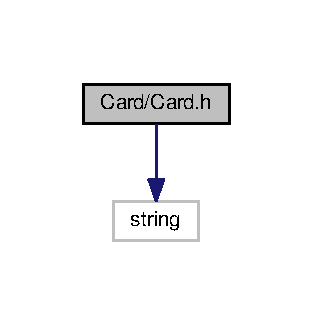
\includegraphics[width=150pt]{Card_8h__incl}
\end{center}
\end{figure}
This graph shows which files directly or indirectly include this file\-:\nopagebreak
\begin{figure}[H]
\begin{center}
\leavevmode
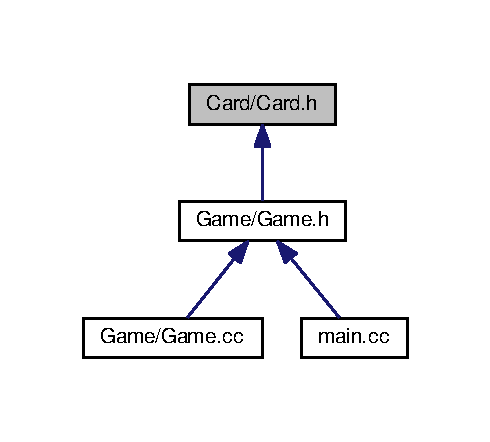
\includegraphics[width=235pt]{Card_8h__dep__incl}
\end{center}
\end{figure}
\subsection*{Classes}
\begin{DoxyCompactItemize}
\item 
class \hyperlink{classCard}{Card}
\end{DoxyCompactItemize}

\hypertarget{Company_8cc}{\section{Company/\-Company.cc File Reference}
\label{Company_8cc}\index{Company/\-Company.\-cc@{Company/\-Company.\-cc}}
}
{\ttfamily \#include $<$cstring$>$}\\*
{\ttfamily \#include $<$cstdlib$>$}\\*
{\ttfamily \#include \char`\"{}Company.\-h\char`\"{}}\\*
Include dependency graph for Company.\-cc\-:
\nopagebreak
\begin{figure}[H]
\begin{center}
\leavevmode
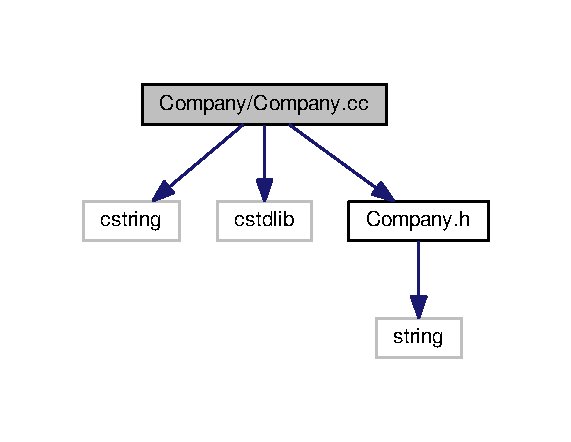
\includegraphics[width=274pt]{Company_8cc__incl}
\end{center}
\end{figure}

\hypertarget{Company_8h}{\section{Company/\-Company.h File Reference}
\label{Company_8h}\index{Company/\-Company.\-h@{Company/\-Company.\-h}}
}
{\ttfamily \#include $<$string$>$}\\*
Include dependency graph for Company.\-h\-:
\nopagebreak
\begin{figure}[H]
\begin{center}
\leavevmode
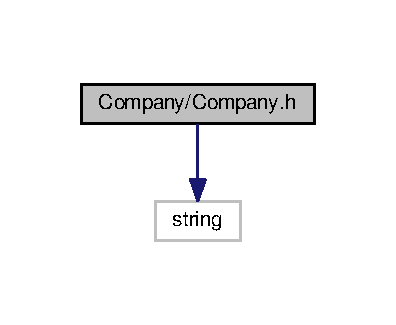
\includegraphics[width=190pt]{Company_8h__incl}
\end{center}
\end{figure}
This graph shows which files directly or indirectly include this file\-:
\nopagebreak
\begin{figure}[H]
\begin{center}
\leavevmode
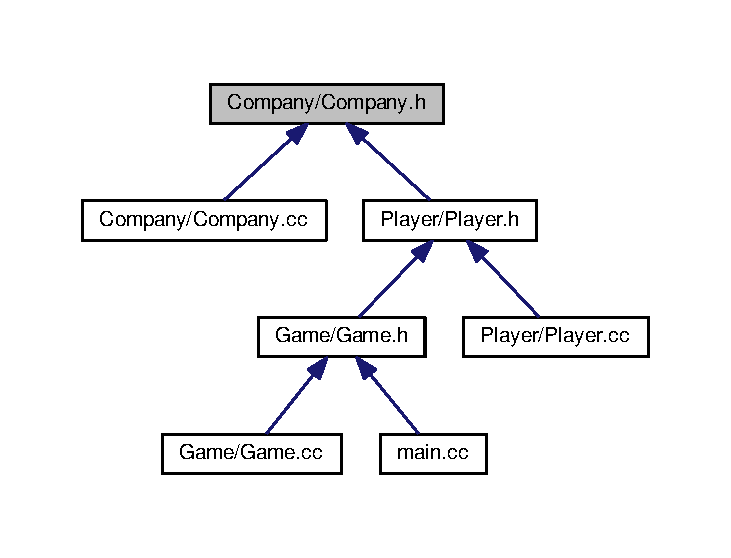
\includegraphics[width=350pt]{Company_8h__dep__incl}
\end{center}
\end{figure}
\subsection*{Classes}
\begin{DoxyCompactItemize}
\item 
class \hyperlink{classCompany}{Company}
\end{DoxyCompactItemize}
\subsection*{Macros}
\begin{DoxyCompactItemize}
\item 
\#define \hyperlink{Company_8h_ace2d0ad84a4d98a49c509063dbbf9a1c}{C\-O\-M\-P\-A\-N\-Y\-\_\-\-P\-R\-I\-C\-E}~500000
\end{DoxyCompactItemize}


\subsection{Macro Definition Documentation}
\hypertarget{Company_8h_ace2d0ad84a4d98a49c509063dbbf9a1c}{\index{Company.\-h@{Company.\-h}!C\-O\-M\-P\-A\-N\-Y\-\_\-\-P\-R\-I\-C\-E@{C\-O\-M\-P\-A\-N\-Y\-\_\-\-P\-R\-I\-C\-E}}
\index{C\-O\-M\-P\-A\-N\-Y\-\_\-\-P\-R\-I\-C\-E@{C\-O\-M\-P\-A\-N\-Y\-\_\-\-P\-R\-I\-C\-E}!Company.h@{Company.\-h}}
\subsubsection[{C\-O\-M\-P\-A\-N\-Y\-\_\-\-P\-R\-I\-C\-E}]{\setlength{\rightskip}{0pt plus 5cm}\#define C\-O\-M\-P\-A\-N\-Y\-\_\-\-P\-R\-I\-C\-E~500000}}\label{Company_8h_ace2d0ad84a4d98a49c509063dbbf9a1c}

\hypertarget{Game_8cc}{\section{Game/\-Game.cc File Reference}
\label{Game_8cc}\index{Game/\-Game.\-cc@{Game/\-Game.\-cc}}
}
{\ttfamily \#include $<$cstdio$>$}\\*
{\ttfamily \#include \char`\"{}Game.\-h\char`\"{}}\\*
Include dependency graph for Game.\-cc\-:\nopagebreak
\begin{figure}[H]
\begin{center}
\leavevmode
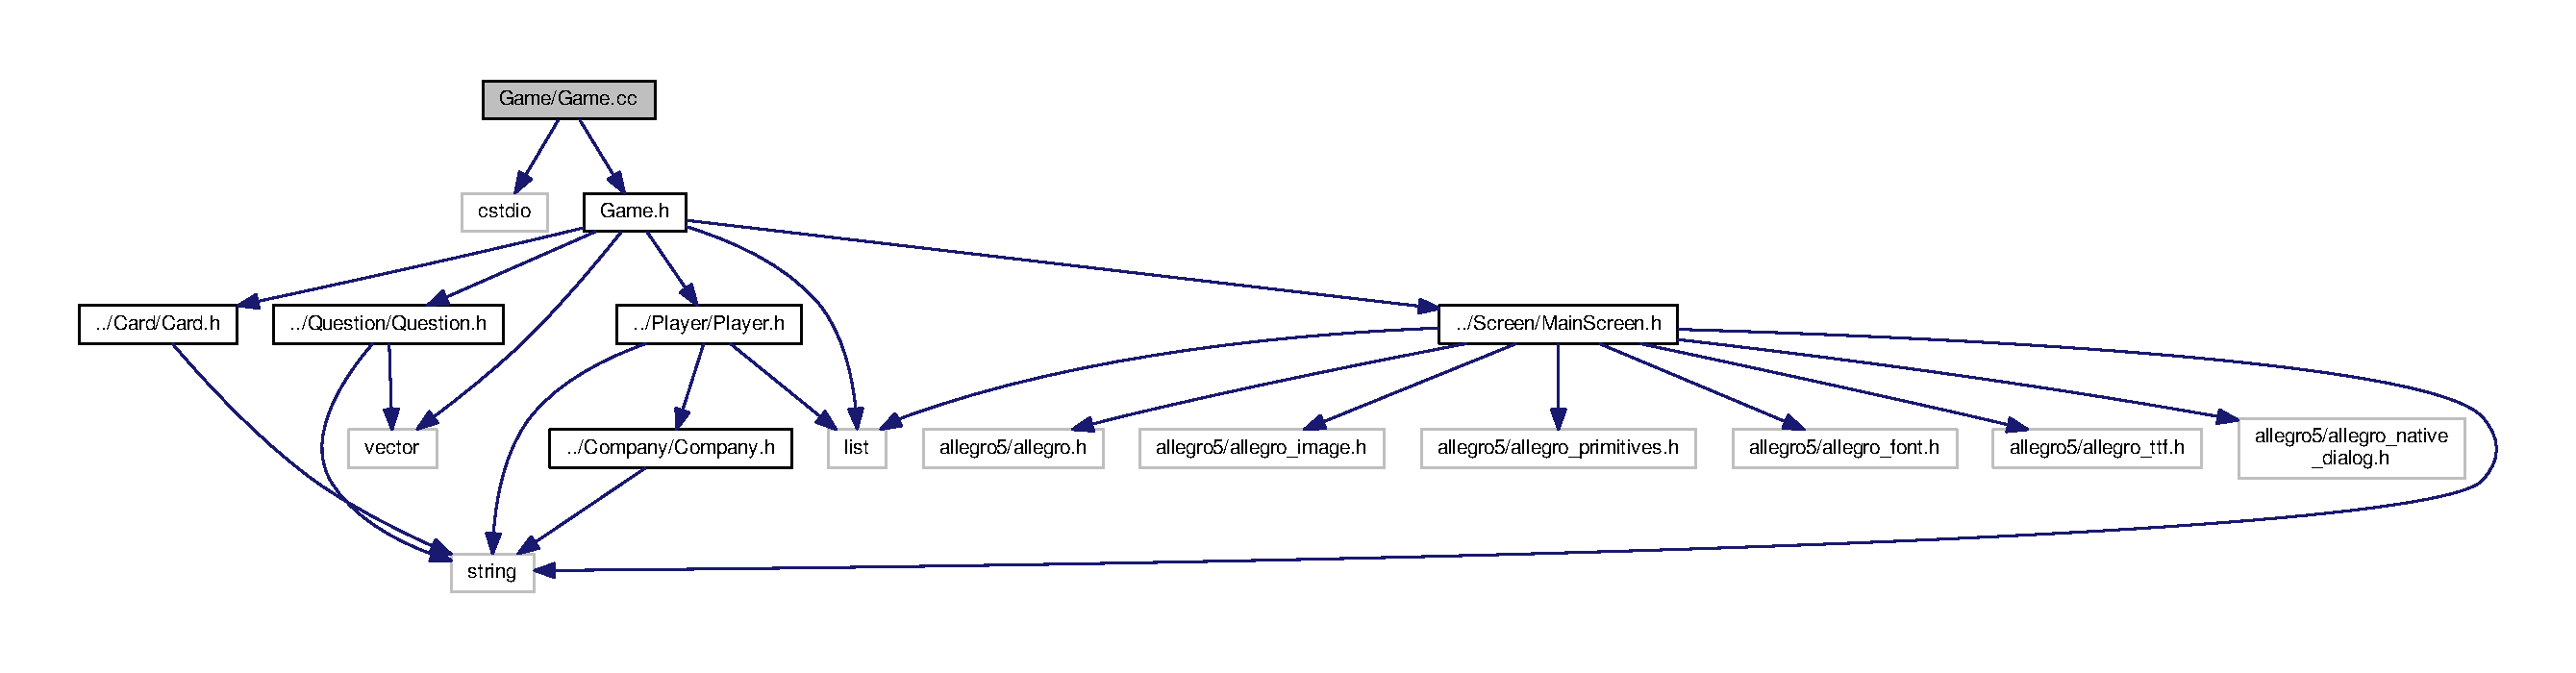
\includegraphics[width=350pt]{Game_8cc__incl}
\end{center}
\end{figure}

\hypertarget{Game_8h}{\section{Game/\-Game.h File Reference}
\label{Game_8h}\index{Game/\-Game.\-h@{Game/\-Game.\-h}}
}
{\ttfamily \#include $<$vector$>$}\\*
{\ttfamily \#include $<$list$>$}\\*
{\ttfamily \#include \char`\"{}../\-Player/\-Player.\-h\char`\"{}}\\*
{\ttfamily \#include \char`\"{}../\-Screen/\-Main\-Screen.\-h\char`\"{}}\\*
{\ttfamily \#include \char`\"{}../\-Question/\-Question.\-h\char`\"{}}\\*
{\ttfamily \#include \char`\"{}../\-Card/\-Card.\-h\char`\"{}}\\*
Include dependency graph for Game.\-h\-:
\nopagebreak
\begin{figure}[H]
\begin{center}
\leavevmode
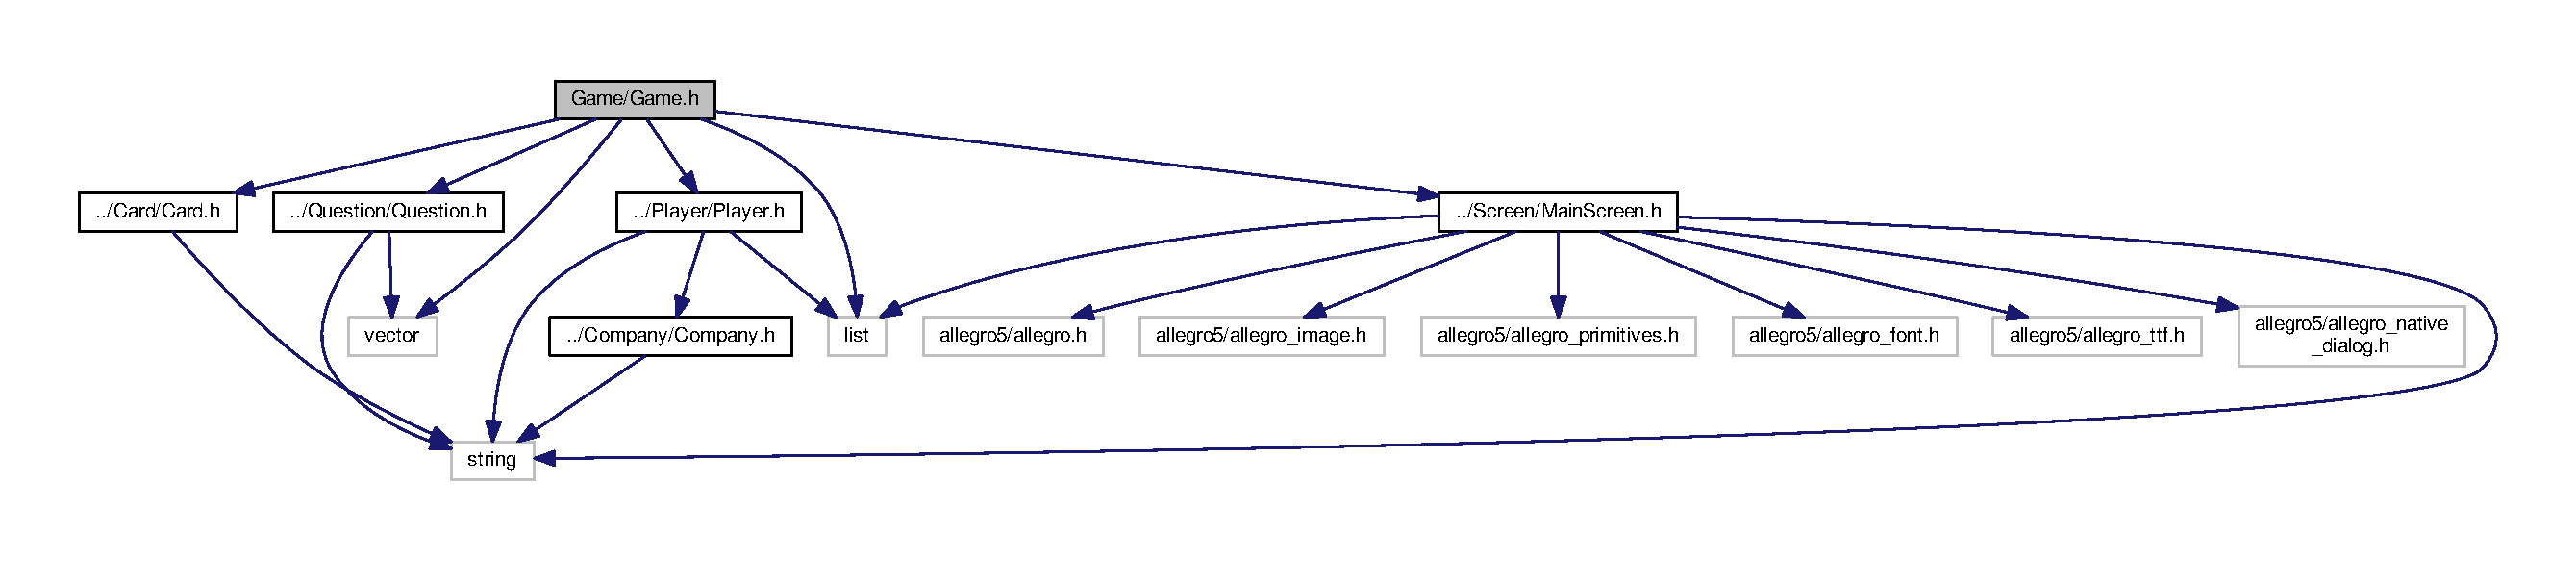
\includegraphics[width=350pt]{Game_8h__incl}
\end{center}
\end{figure}
This graph shows which files directly or indirectly include this file\-:
\nopagebreak
\begin{figure}[H]
\begin{center}
\leavevmode
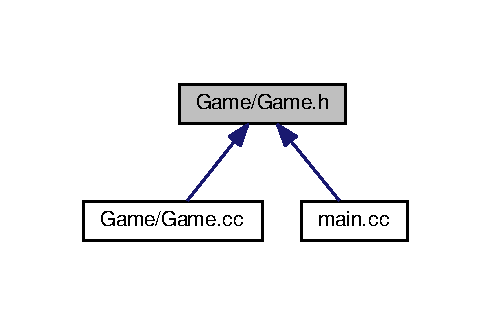
\includegraphics[width=235pt]{Game_8h__dep__incl}
\end{center}
\end{figure}
\subsection*{Classes}
\begin{DoxyCompactItemize}
\item 
class \hyperlink{classGame}{Game}
\end{DoxyCompactItemize}

\hypertarget{main_8cc}{\section{main.\-cc File Reference}
\label{main_8cc}\index{main.\-cc@{main.\-cc}}
}
{\ttfamily \#include $<$allegro5/allegro.\-h$>$}\\*
{\ttfamily \#include $<$allegro5/allegro\-\_\-image.\-h$>$}\\*
{\ttfamily \#include $<$allegro5/allegro\-\_\-primitives.\-h$>$}\\*
{\ttfamily \#include $<$allegro5/allegro\-\_\-font.\-h$>$}\\*
{\ttfamily \#include $<$allegro5/allegro\-\_\-ttf.\-h$>$}\\*
{\ttfamily \#include $<$allegro5/allegro\-\_\-native\-\_\-dialog.\-h$>$}\\*
{\ttfamily \#include $<$list$>$}\\*
{\ttfamily \#include $<$cstdio$>$}\\*
{\ttfamily \#include \char`\"{}Game/\-Game.\-h\char`\"{}}\\*
Include dependency graph for main.\-cc\-:
\nopagebreak
\begin{figure}[H]
\begin{center}
\leavevmode
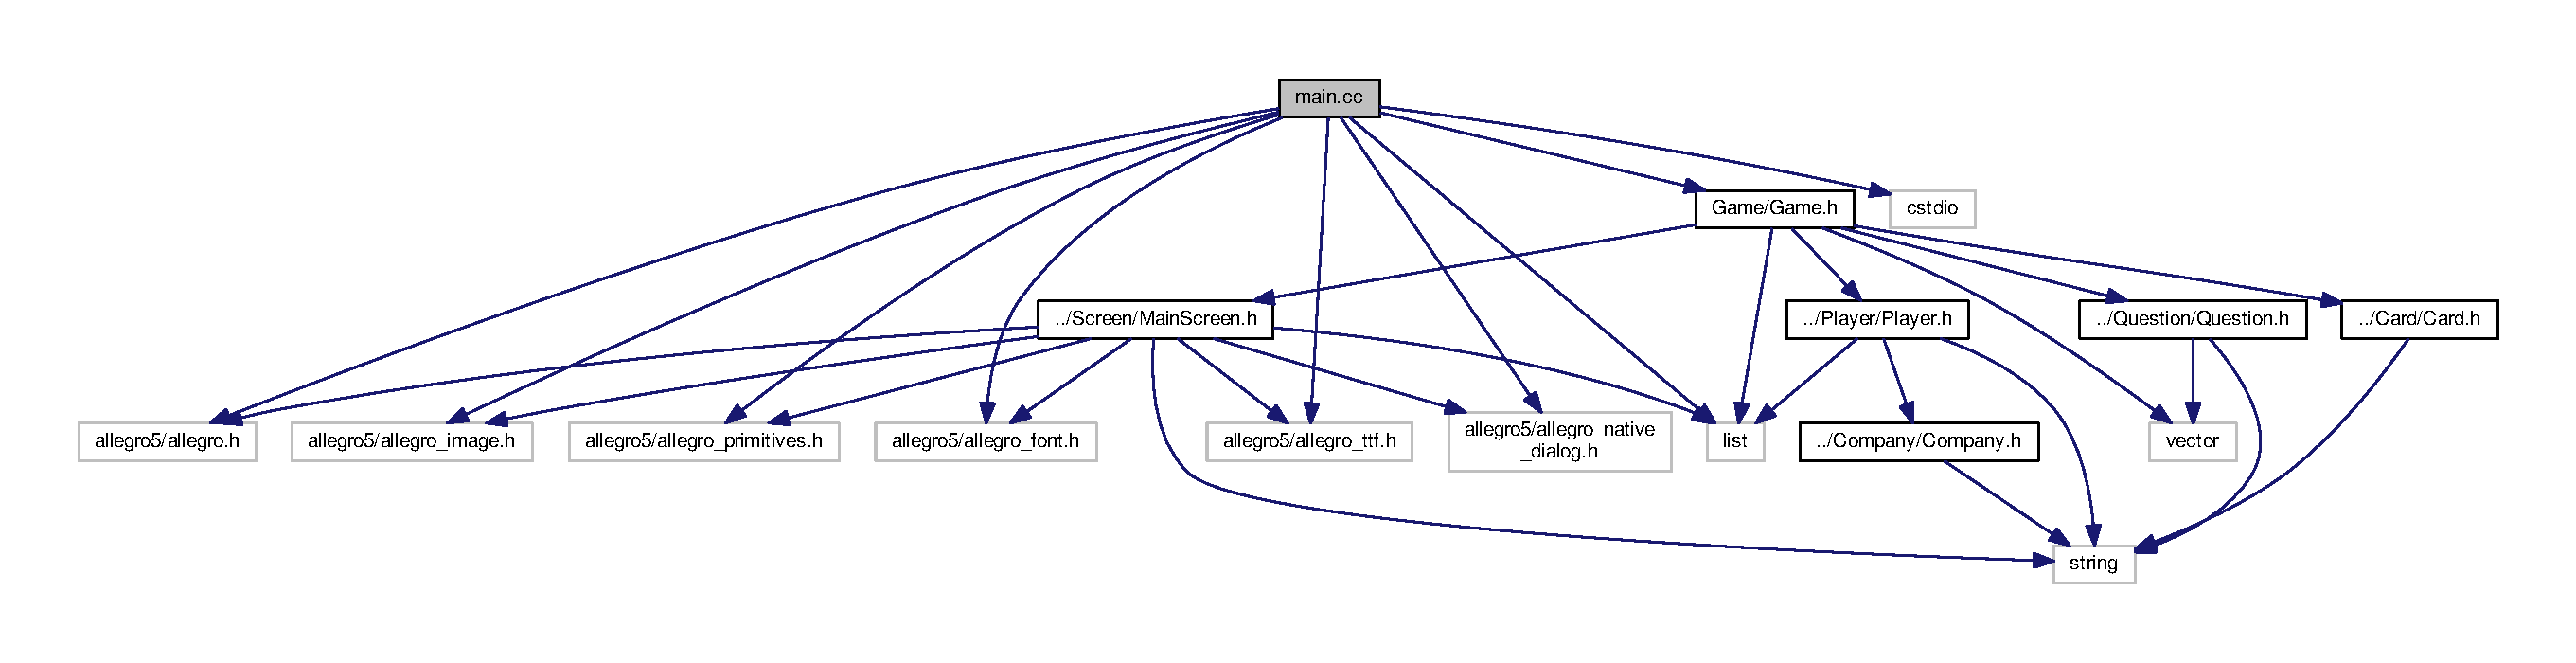
\includegraphics[width=350pt]{main_8cc__incl}
\end{center}
\end{figure}
\subsection*{Functions}
\begin{DoxyCompactItemize}
\item 
int \hyperlink{main_8cc_ae66f6b31b5ad750f1fe042a706a4e3d4}{main} ()
\end{DoxyCompactItemize}


\subsection{Function Documentation}
\hypertarget{main_8cc_ae66f6b31b5ad750f1fe042a706a4e3d4}{\index{main.\-cc@{main.\-cc}!main@{main}}
\index{main@{main}!main.cc@{main.\-cc}}
\subsubsection[{main}]{\setlength{\rightskip}{0pt plus 5cm}int main (
\begin{DoxyParamCaption}
{}
\end{DoxyParamCaption}
)}}\label{main_8cc_ae66f6b31b5ad750f1fe042a706a4e3d4}

\begin{DoxyCode}
15 \{
16     printf(\textcolor{stringliteral}{"Initializing Allegro...\(\backslash\)n"});
17         \textcolor{keywordflow}{if} (!al\_init())
18         \{
19                 fprintf(stderr, \textcolor{stringliteral}{"failed to initialize allegro!\(\backslash\)n"});
20                 \textcolor{keywordflow}{return} EXIT\_FAILURE;
21         \}
22         al\_init\_native\_dialog\_addon();
23         al\_init\_image\_addon();
24         al\_init\_primitives\_addon();
25         al\_init\_font\_addon();
26         al\_init\_ttf\_addon();
27         al\_install\_mouse();
28         srand(time(NULL));
29 
30     printf(\textcolor{stringliteral}{"Showing configuration screen...\(\backslash\)n"});
31     \textcolor{comment}{//TODO: Call configuration screen and get info regarding players and stuff}
32 
33     list< pair<pair<const char*, const char*>, \textcolor{keyword}{const} \textcolor{keywordtype}{char}*> > infoPlayers;
34     infoPlayers.push\_back(pair<pair<const char*, const char*>, \textcolor{keyword}{const} \textcolor{keywordtype}{char}*>(pair<const char*, const char*>(\textcolor{stringliteral}{
      "João da Silva"}, \textcolor{stringliteral}{"XP"}), 
35         \textcolor{stringliteral}{"../misc/images/avatar.jpg"}));
36     infoPlayers.push\_back(pair<pair<const char*, const char*>, \textcolor{keyword}{const} \textcolor{keywordtype}{char}*>(pair<const char*, const char*>(\textcolor{stringliteral}{
      "Maria Souza"}, \textcolor{stringliteral}{"Scrum"}), 
37         \textcolor{stringliteral}{"../misc/images/hebe.jpg"}));
38     infoPlayers.push\_back(pair<pair<const char*, const char*>, \textcolor{keyword}{const} \textcolor{keywordtype}{char}*>(pair<const char*, const char*>(\textcolor{stringliteral}{
      "Antônio Alberto"}, \textcolor{stringliteral}{"Praxis"}), 
39         \textcolor{stringliteral}{"../misc/images/gugu.jpg"}));
40     infoPlayers.push\_back(pair<pair<const char*, const char*>, \textcolor{keyword}{const} \textcolor{keywordtype}{char}*>(pair<const char*, const char*>(\textcolor{stringliteral}{
      "Clara Nunes"}, \textcolor{stringliteral}{"Kanban"}), 
41         \textcolor{stringliteral}{"../misc/images/xuxa.jpg"}));
42 
43     printf(\textcolor{stringliteral}{"Starting game...\(\backslash\)n"});
44     \hyperlink{classGame}{Game} game(infoPlayers, 5);
45     game.startGame();
46 
47         \textcolor{keywordflow}{return} EXIT\_SUCCESS;
48 \}
\end{DoxyCode}


Here is the call graph for this function\-:
\nopagebreak
\begin{figure}[H]
\begin{center}
\leavevmode
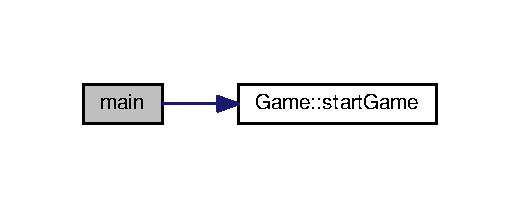
\includegraphics[width=250pt]{main_8cc_ae66f6b31b5ad750f1fe042a706a4e3d4_cgraph}
\end{center}
\end{figure}



\hypertarget{Player_8cc}{\section{Player/\-Player.cc File Reference}
\label{Player_8cc}\index{Player/\-Player.\-cc@{Player/\-Player.\-cc}}
}
{\ttfamily \#include $<$cstdlib$>$}\\*
{\ttfamily \#include $<$cstring$>$}\\*
{\ttfamily \#include \char`\"{}Player.\-h\char`\"{}}\\*
Include dependency graph for Player.\-cc\-:\nopagebreak
\begin{figure}[H]
\begin{center}
\leavevmode
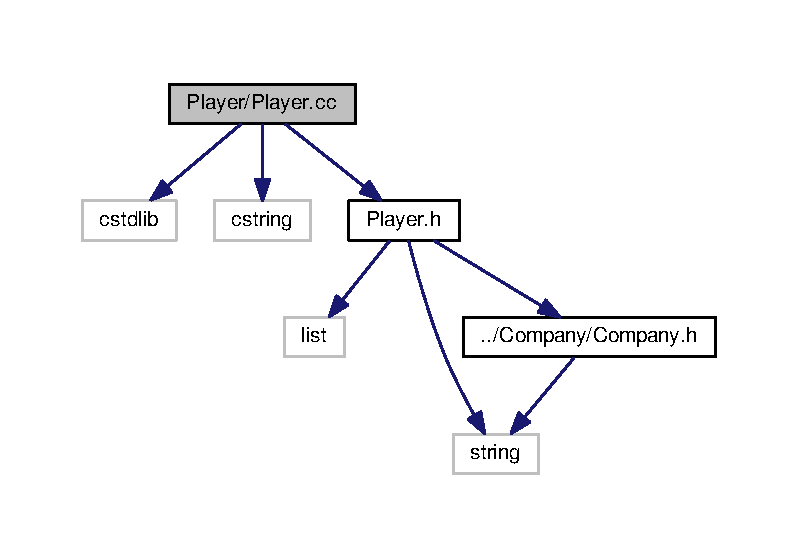
\includegraphics[width=350pt]{Player_8cc__incl}
\end{center}
\end{figure}

\hypertarget{Player_8h}{\section{Player/\-Player.h File Reference}
\label{Player_8h}\index{Player/\-Player.\-h@{Player/\-Player.\-h}}
}
{\ttfamily \#include $<$list$>$}\\*
{\ttfamily \#include $<$string$>$}\\*
{\ttfamily \#include \char`\"{}../\-Company/\-Company.\-h\char`\"{}}\\*
Include dependency graph for Player.\-h\-:\nopagebreak
\begin{figure}[H]
\begin{center}
\leavevmode
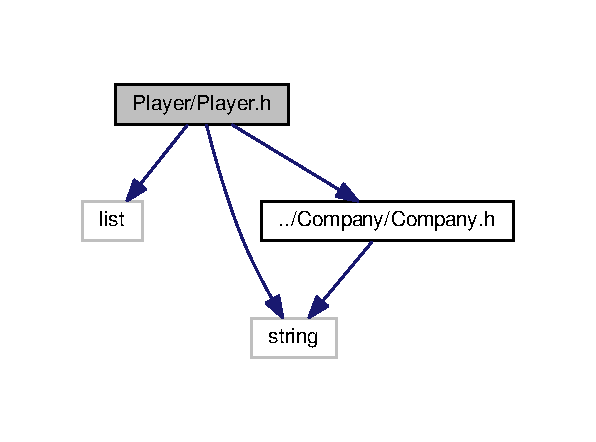
\includegraphics[width=286pt]{Player_8h__incl}
\end{center}
\end{figure}
This graph shows which files directly or indirectly include this file\-:\nopagebreak
\begin{figure}[H]
\begin{center}
\leavevmode
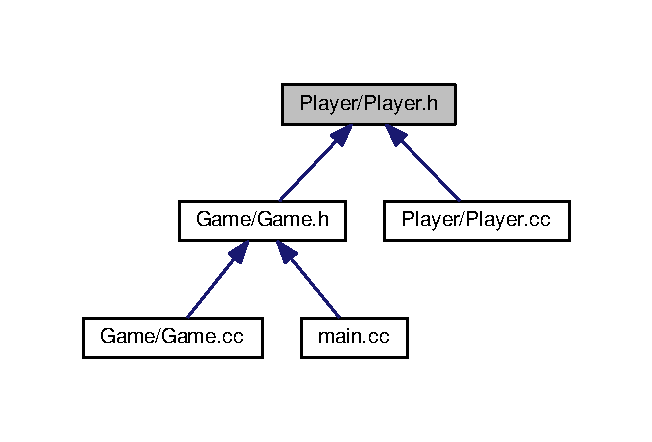
\includegraphics[width=313pt]{Player_8h__dep__incl}
\end{center}
\end{figure}
\subsection*{Classes}
\begin{DoxyCompactItemize}
\item 
class \hyperlink{classPlayer}{Player}
\end{DoxyCompactItemize}
\subsection*{Macros}
\begin{DoxyCompactItemize}
\item 
\#define \hyperlink{Player_8h_a984027001c10072051bf999609f9167d}{I\-N\-I\-T\-I\-A\-L\-\_\-\-R\-E\-S\-O\-U\-R\-C\-E\-S}~2000000
\end{DoxyCompactItemize}


\subsection{Macro Definition Documentation}
\hypertarget{Player_8h_a984027001c10072051bf999609f9167d}{\index{Player.\-h@{Player.\-h}!I\-N\-I\-T\-I\-A\-L\-\_\-\-R\-E\-S\-O\-U\-R\-C\-E\-S@{I\-N\-I\-T\-I\-A\-L\-\_\-\-R\-E\-S\-O\-U\-R\-C\-E\-S}}
\index{I\-N\-I\-T\-I\-A\-L\-\_\-\-R\-E\-S\-O\-U\-R\-C\-E\-S@{I\-N\-I\-T\-I\-A\-L\-\_\-\-R\-E\-S\-O\-U\-R\-C\-E\-S}!Player.h@{Player.\-h}}
\subsubsection[{I\-N\-I\-T\-I\-A\-L\-\_\-\-R\-E\-S\-O\-U\-R\-C\-E\-S}]{\setlength{\rightskip}{0pt plus 5cm}\#define I\-N\-I\-T\-I\-A\-L\-\_\-\-R\-E\-S\-O\-U\-R\-C\-E\-S~2000000}}\label{Player_8h_a984027001c10072051bf999609f9167d}

\hypertarget{Question_8cc}{\section{Question/\-Question.cc File Reference}
\label{Question_8cc}\index{Question/\-Question.\-cc@{Question/\-Question.\-cc}}
}

\hypertarget{Question_8h}{\section{Question/\-Question.h File Reference}
\label{Question_8h}\index{Question/\-Question.\-h@{Question/\-Question.\-h}}
}
{\ttfamily \#include $<$string$>$}\\*
{\ttfamily \#include $<$vector$>$}\\*
Include dependency graph for Question.\-h\-:
\nopagebreak
\begin{figure}[H]
\begin{center}
\leavevmode
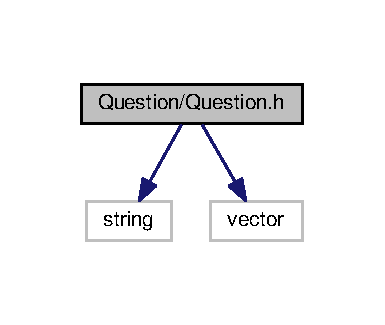
\includegraphics[width=185pt]{Question_8h__incl}
\end{center}
\end{figure}
This graph shows which files directly or indirectly include this file\-:
\nopagebreak
\begin{figure}[H]
\begin{center}
\leavevmode
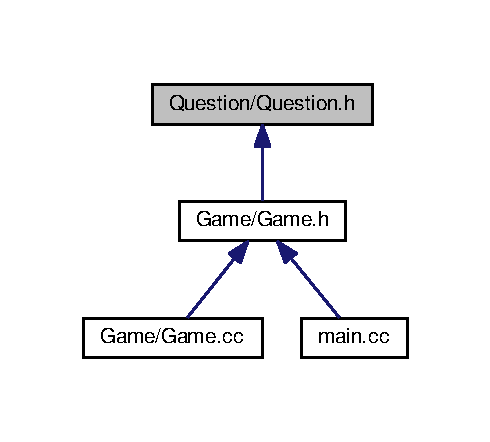
\includegraphics[width=235pt]{Question_8h__dep__incl}
\end{center}
\end{figure}
\subsection*{Classes}
\begin{DoxyCompactItemize}
\item 
class \hyperlink{classQuestion}{Question}
\end{DoxyCompactItemize}

\hypertarget{MainScreen_8cc}{\section{Screen/\-Main\-Screen.cc File Reference}
\label{MainScreen_8cc}\index{Screen/\-Main\-Screen.\-cc@{Screen/\-Main\-Screen.\-cc}}
}
{\ttfamily \#include $<$stdio.\-h$>$}\\*
{\ttfamily \#include $<$math.\-h$>$}\\*
{\ttfamily \#include $<$time.\-h$>$}\\*
{\ttfamily \#include $<$list$>$}\\*
{\ttfamily \#include \char`\"{}Main\-Screen.\-h\char`\"{}}\\*
Include dependency graph for Main\-Screen.\-cc\-:
\nopagebreak
\begin{figure}[H]
\begin{center}
\leavevmode
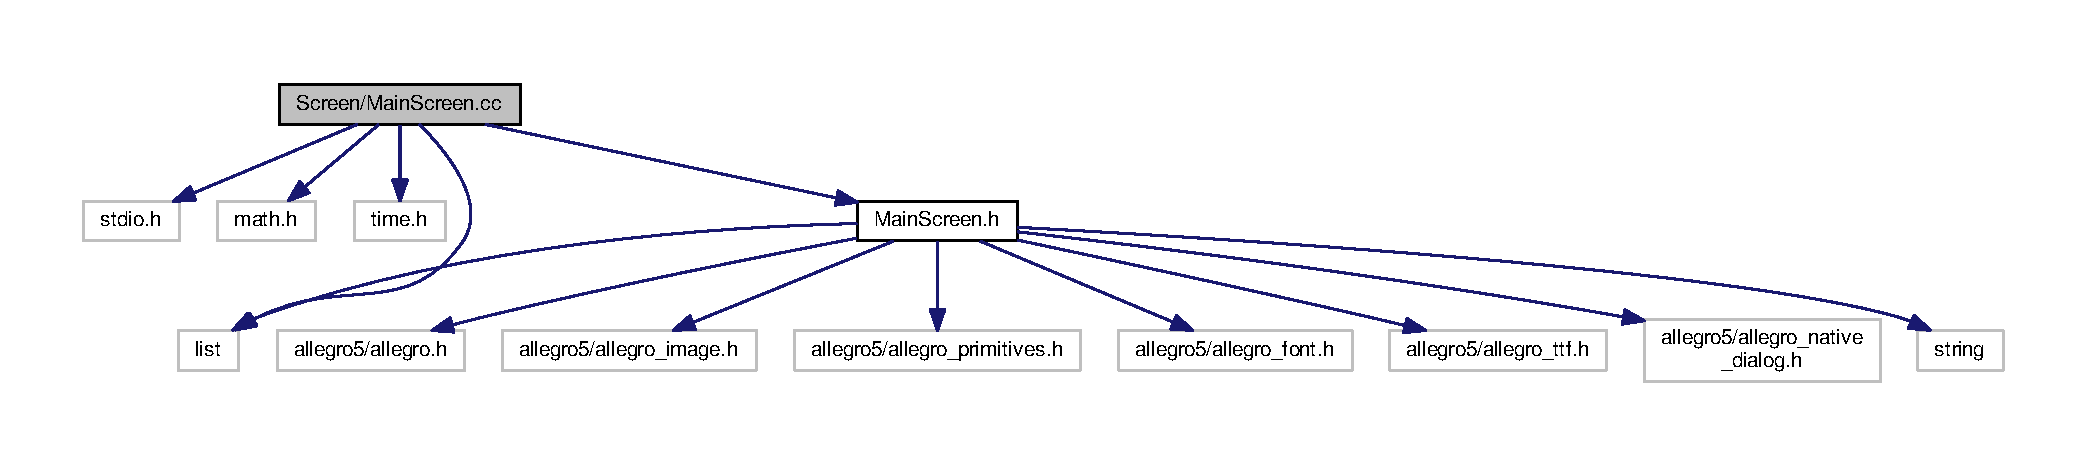
\includegraphics[width=350pt]{MainScreen_8cc__incl}
\end{center}
\end{figure}

\hypertarget{MainScreen_8h}{\section{Screen/\-Main\-Screen.h File Reference}
\label{MainScreen_8h}\index{Screen/\-Main\-Screen.\-h@{Screen/\-Main\-Screen.\-h}}
}
{\ttfamily \#include $<$allegro5/allegro.\-h$>$}\\*
{\ttfamily \#include $<$allegro5/allegro\-\_\-image.\-h$>$}\\*
{\ttfamily \#include $<$allegro5/allegro\-\_\-primitives.\-h$>$}\\*
{\ttfamily \#include $<$allegro5/allegro\-\_\-font.\-h$>$}\\*
{\ttfamily \#include $<$allegro5/allegro\-\_\-ttf.\-h$>$}\\*
{\ttfamily \#include $<$allegro5/allegro\-\_\-native\-\_\-dialog.\-h$>$}\\*
{\ttfamily \#include $<$list$>$}\\*
{\ttfamily \#include $<$string$>$}\\*
Include dependency graph for Main\-Screen.\-h\-:
\nopagebreak
\begin{figure}[H]
\begin{center}
\leavevmode
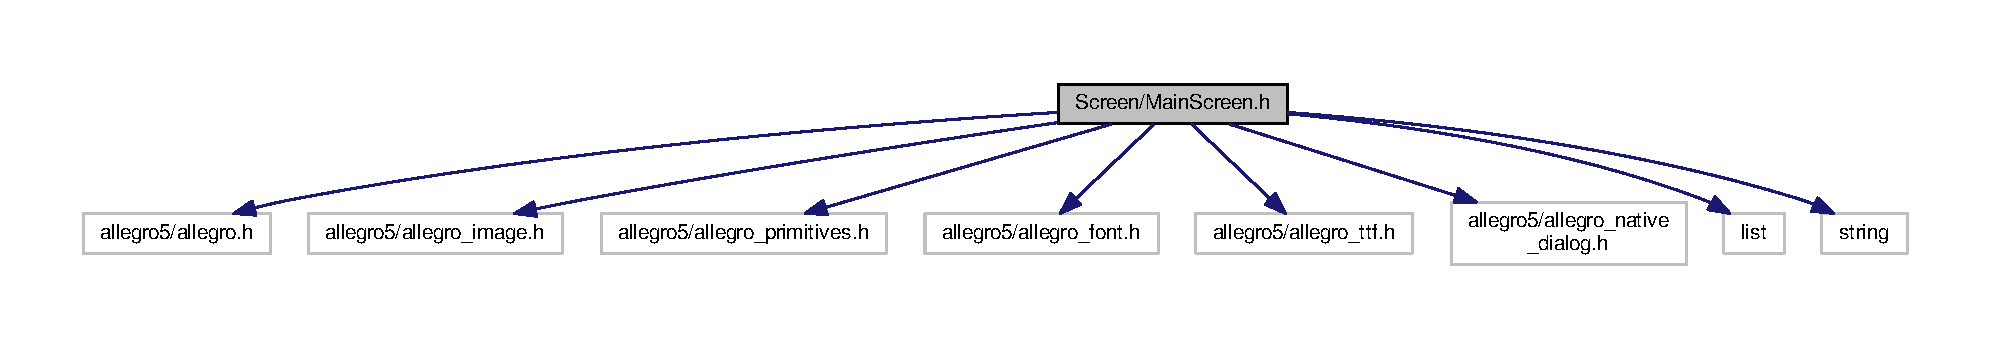
\includegraphics[width=350pt]{MainScreen_8h__incl}
\end{center}
\end{figure}
This graph shows which files directly or indirectly include this file\-:
\nopagebreak
\begin{figure}[H]
\begin{center}
\leavevmode
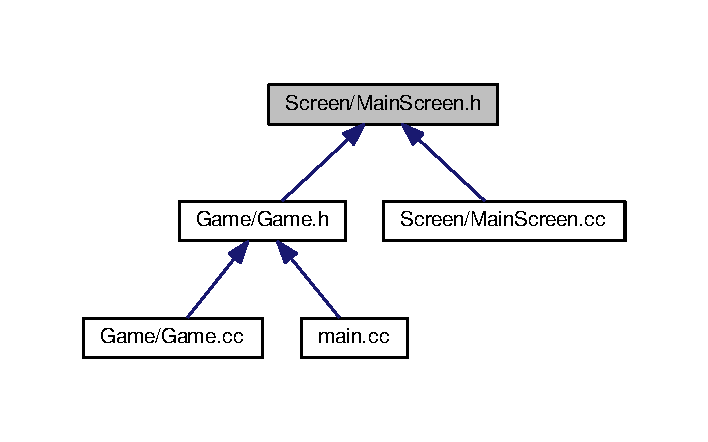
\includegraphics[width=340pt]{MainScreen_8h__dep__incl}
\end{center}
\end{figure}
\subsection*{Classes}
\begin{DoxyCompactItemize}
\item 
class \hyperlink{classMainScreen}{Main\-Screen}
\end{DoxyCompactItemize}
\subsection*{Macros}
\begin{DoxyCompactItemize}
\item 
\#define \hyperlink{MainScreen_8h_a317b5109da7c376133ac189c84b42640}{H\-O\-R\-\_\-\-L\-I\-N\-E\-\_\-\-I\-N\-F\-O\-\_\-\-P\-L\-A\-Y\-E\-R\-\_\-\-H\-E\-I\-G\-H\-T}~0.\-65
\item 
\#define \hyperlink{MainScreen_8h_a7e18b3decda36fa1ea88693a2e3db612}{H\-O\-R\-\_\-\-L\-I\-N\-E\-\_\-\-R\-O\-U\-N\-D\-S\-\_\-\-H\-E\-I\-G\-H\-T}~0.\-05
\item 
\#define \hyperlink{MainScreen_8h_a95248267b1e9860a49b38b91d6060ac3}{V\-E\-R\-T\-\_\-\-L\-I\-N\-E\-\_\-\-P\-L\-A\-Y\-E\-R\-S\-\_\-\-W\-I\-D\-T\-H}~0.\-7
\item 
\#define \hyperlink{MainScreen_8h_a85b60dfcd77a2e87a8c3cad02c69fd57}{V\-E\-R\-T\-\_\-\-L\-I\-N\-E\-\_\-\-A\-V\-A\-T\-A\-R\-\_\-\-W\-I\-D\-T\-H}~0.\-15
\item 
\#define \hyperlink{MainScreen_8h_a18c12502cb14f5c3534be1cd0abff393}{I\-N\-V\-E\-N\-T\-O\-R\-Y\-\_\-\-H\-E\-I\-G\-H\-T\-\_\-\-P\-O\-S}~0.\-73
\item 
\#define \hyperlink{MainScreen_8h_a25d2fe10be4c43346aba598e8b6011cf}{I\-N\-V\-E\-N\-T\-O\-R\-Y\-\_\-\-W\-I\-D\-T\-H\-\_\-\-P\-O\-S}~0.\-65
\item 
\#define \hyperlink{MainScreen_8h_a59ff38ce73af72905372fda08af0e6ef}{I\-N\-V\-E\-N\-T\-O\-R\-Y\-\_\-\-H\-E\-I\-G\-H\-T}~0.\-25
\item 
\#define \hyperlink{MainScreen_8h_a2da9fa54c9fc60662dbda40b0139a1e9}{I\-N\-V\-E\-N\-T\-O\-R\-Y\-\_\-\-W\-I\-D\-T\-H}~0.\-3
\item 
\#define \hyperlink{MainScreen_8h_adeacbb83e11064c564e0730c739d4322}{I\-N\-V\-E\-N\-T\-O\-R\-Y\-\_\-\-T\-I\-T\-L\-E\-\_\-\-W\-I\-D\-T\-H}~0.\-75
\item 
\#define \hyperlink{MainScreen_8h_a287d362f882751508f72d74b3df95386}{I\-N\-V\-E\-N\-T\-O\-R\-Y\-\_\-\-T\-I\-T\-L\-E\-\_\-\-H\-E\-I\-G\-H\-T}~0.\-68
\end{DoxyCompactItemize}


\subsection{Macro Definition Documentation}
\hypertarget{MainScreen_8h_a317b5109da7c376133ac189c84b42640}{\index{Main\-Screen.\-h@{Main\-Screen.\-h}!H\-O\-R\-\_\-\-L\-I\-N\-E\-\_\-\-I\-N\-F\-O\-\_\-\-P\-L\-A\-Y\-E\-R\-\_\-\-H\-E\-I\-G\-H\-T@{H\-O\-R\-\_\-\-L\-I\-N\-E\-\_\-\-I\-N\-F\-O\-\_\-\-P\-L\-A\-Y\-E\-R\-\_\-\-H\-E\-I\-G\-H\-T}}
\index{H\-O\-R\-\_\-\-L\-I\-N\-E\-\_\-\-I\-N\-F\-O\-\_\-\-P\-L\-A\-Y\-E\-R\-\_\-\-H\-E\-I\-G\-H\-T@{H\-O\-R\-\_\-\-L\-I\-N\-E\-\_\-\-I\-N\-F\-O\-\_\-\-P\-L\-A\-Y\-E\-R\-\_\-\-H\-E\-I\-G\-H\-T}!MainScreen.h@{Main\-Screen.\-h}}
\subsubsection[{H\-O\-R\-\_\-\-L\-I\-N\-E\-\_\-\-I\-N\-F\-O\-\_\-\-P\-L\-A\-Y\-E\-R\-\_\-\-H\-E\-I\-G\-H\-T}]{\setlength{\rightskip}{0pt plus 5cm}\#define H\-O\-R\-\_\-\-L\-I\-N\-E\-\_\-\-I\-N\-F\-O\-\_\-\-P\-L\-A\-Y\-E\-R\-\_\-\-H\-E\-I\-G\-H\-T~0.\-65}}\label{MainScreen_8h_a317b5109da7c376133ac189c84b42640}
\hypertarget{MainScreen_8h_a7e18b3decda36fa1ea88693a2e3db612}{\index{Main\-Screen.\-h@{Main\-Screen.\-h}!H\-O\-R\-\_\-\-L\-I\-N\-E\-\_\-\-R\-O\-U\-N\-D\-S\-\_\-\-H\-E\-I\-G\-H\-T@{H\-O\-R\-\_\-\-L\-I\-N\-E\-\_\-\-R\-O\-U\-N\-D\-S\-\_\-\-H\-E\-I\-G\-H\-T}}
\index{H\-O\-R\-\_\-\-L\-I\-N\-E\-\_\-\-R\-O\-U\-N\-D\-S\-\_\-\-H\-E\-I\-G\-H\-T@{H\-O\-R\-\_\-\-L\-I\-N\-E\-\_\-\-R\-O\-U\-N\-D\-S\-\_\-\-H\-E\-I\-G\-H\-T}!MainScreen.h@{Main\-Screen.\-h}}
\subsubsection[{H\-O\-R\-\_\-\-L\-I\-N\-E\-\_\-\-R\-O\-U\-N\-D\-S\-\_\-\-H\-E\-I\-G\-H\-T}]{\setlength{\rightskip}{0pt plus 5cm}\#define H\-O\-R\-\_\-\-L\-I\-N\-E\-\_\-\-R\-O\-U\-N\-D\-S\-\_\-\-H\-E\-I\-G\-H\-T~0.\-05}}\label{MainScreen_8h_a7e18b3decda36fa1ea88693a2e3db612}
\hypertarget{MainScreen_8h_a59ff38ce73af72905372fda08af0e6ef}{\index{Main\-Screen.\-h@{Main\-Screen.\-h}!I\-N\-V\-E\-N\-T\-O\-R\-Y\-\_\-\-H\-E\-I\-G\-H\-T@{I\-N\-V\-E\-N\-T\-O\-R\-Y\-\_\-\-H\-E\-I\-G\-H\-T}}
\index{I\-N\-V\-E\-N\-T\-O\-R\-Y\-\_\-\-H\-E\-I\-G\-H\-T@{I\-N\-V\-E\-N\-T\-O\-R\-Y\-\_\-\-H\-E\-I\-G\-H\-T}!MainScreen.h@{Main\-Screen.\-h}}
\subsubsection[{I\-N\-V\-E\-N\-T\-O\-R\-Y\-\_\-\-H\-E\-I\-G\-H\-T}]{\setlength{\rightskip}{0pt plus 5cm}\#define I\-N\-V\-E\-N\-T\-O\-R\-Y\-\_\-\-H\-E\-I\-G\-H\-T~0.\-25}}\label{MainScreen_8h_a59ff38ce73af72905372fda08af0e6ef}
\hypertarget{MainScreen_8h_a18c12502cb14f5c3534be1cd0abff393}{\index{Main\-Screen.\-h@{Main\-Screen.\-h}!I\-N\-V\-E\-N\-T\-O\-R\-Y\-\_\-\-H\-E\-I\-G\-H\-T\-\_\-\-P\-O\-S@{I\-N\-V\-E\-N\-T\-O\-R\-Y\-\_\-\-H\-E\-I\-G\-H\-T\-\_\-\-P\-O\-S}}
\index{I\-N\-V\-E\-N\-T\-O\-R\-Y\-\_\-\-H\-E\-I\-G\-H\-T\-\_\-\-P\-O\-S@{I\-N\-V\-E\-N\-T\-O\-R\-Y\-\_\-\-H\-E\-I\-G\-H\-T\-\_\-\-P\-O\-S}!MainScreen.h@{Main\-Screen.\-h}}
\subsubsection[{I\-N\-V\-E\-N\-T\-O\-R\-Y\-\_\-\-H\-E\-I\-G\-H\-T\-\_\-\-P\-O\-S}]{\setlength{\rightskip}{0pt plus 5cm}\#define I\-N\-V\-E\-N\-T\-O\-R\-Y\-\_\-\-H\-E\-I\-G\-H\-T\-\_\-\-P\-O\-S~0.\-73}}\label{MainScreen_8h_a18c12502cb14f5c3534be1cd0abff393}
\hypertarget{MainScreen_8h_a287d362f882751508f72d74b3df95386}{\index{Main\-Screen.\-h@{Main\-Screen.\-h}!I\-N\-V\-E\-N\-T\-O\-R\-Y\-\_\-\-T\-I\-T\-L\-E\-\_\-\-H\-E\-I\-G\-H\-T@{I\-N\-V\-E\-N\-T\-O\-R\-Y\-\_\-\-T\-I\-T\-L\-E\-\_\-\-H\-E\-I\-G\-H\-T}}
\index{I\-N\-V\-E\-N\-T\-O\-R\-Y\-\_\-\-T\-I\-T\-L\-E\-\_\-\-H\-E\-I\-G\-H\-T@{I\-N\-V\-E\-N\-T\-O\-R\-Y\-\_\-\-T\-I\-T\-L\-E\-\_\-\-H\-E\-I\-G\-H\-T}!MainScreen.h@{Main\-Screen.\-h}}
\subsubsection[{I\-N\-V\-E\-N\-T\-O\-R\-Y\-\_\-\-T\-I\-T\-L\-E\-\_\-\-H\-E\-I\-G\-H\-T}]{\setlength{\rightskip}{0pt plus 5cm}\#define I\-N\-V\-E\-N\-T\-O\-R\-Y\-\_\-\-T\-I\-T\-L\-E\-\_\-\-H\-E\-I\-G\-H\-T~0.\-68}}\label{MainScreen_8h_a287d362f882751508f72d74b3df95386}
\hypertarget{MainScreen_8h_adeacbb83e11064c564e0730c739d4322}{\index{Main\-Screen.\-h@{Main\-Screen.\-h}!I\-N\-V\-E\-N\-T\-O\-R\-Y\-\_\-\-T\-I\-T\-L\-E\-\_\-\-W\-I\-D\-T\-H@{I\-N\-V\-E\-N\-T\-O\-R\-Y\-\_\-\-T\-I\-T\-L\-E\-\_\-\-W\-I\-D\-T\-H}}
\index{I\-N\-V\-E\-N\-T\-O\-R\-Y\-\_\-\-T\-I\-T\-L\-E\-\_\-\-W\-I\-D\-T\-H@{I\-N\-V\-E\-N\-T\-O\-R\-Y\-\_\-\-T\-I\-T\-L\-E\-\_\-\-W\-I\-D\-T\-H}!MainScreen.h@{Main\-Screen.\-h}}
\subsubsection[{I\-N\-V\-E\-N\-T\-O\-R\-Y\-\_\-\-T\-I\-T\-L\-E\-\_\-\-W\-I\-D\-T\-H}]{\setlength{\rightskip}{0pt plus 5cm}\#define I\-N\-V\-E\-N\-T\-O\-R\-Y\-\_\-\-T\-I\-T\-L\-E\-\_\-\-W\-I\-D\-T\-H~0.\-75}}\label{MainScreen_8h_adeacbb83e11064c564e0730c739d4322}
\hypertarget{MainScreen_8h_a2da9fa54c9fc60662dbda40b0139a1e9}{\index{Main\-Screen.\-h@{Main\-Screen.\-h}!I\-N\-V\-E\-N\-T\-O\-R\-Y\-\_\-\-W\-I\-D\-T\-H@{I\-N\-V\-E\-N\-T\-O\-R\-Y\-\_\-\-W\-I\-D\-T\-H}}
\index{I\-N\-V\-E\-N\-T\-O\-R\-Y\-\_\-\-W\-I\-D\-T\-H@{I\-N\-V\-E\-N\-T\-O\-R\-Y\-\_\-\-W\-I\-D\-T\-H}!MainScreen.h@{Main\-Screen.\-h}}
\subsubsection[{I\-N\-V\-E\-N\-T\-O\-R\-Y\-\_\-\-W\-I\-D\-T\-H}]{\setlength{\rightskip}{0pt plus 5cm}\#define I\-N\-V\-E\-N\-T\-O\-R\-Y\-\_\-\-W\-I\-D\-T\-H~0.\-3}}\label{MainScreen_8h_a2da9fa54c9fc60662dbda40b0139a1e9}
\hypertarget{MainScreen_8h_a25d2fe10be4c43346aba598e8b6011cf}{\index{Main\-Screen.\-h@{Main\-Screen.\-h}!I\-N\-V\-E\-N\-T\-O\-R\-Y\-\_\-\-W\-I\-D\-T\-H\-\_\-\-P\-O\-S@{I\-N\-V\-E\-N\-T\-O\-R\-Y\-\_\-\-W\-I\-D\-T\-H\-\_\-\-P\-O\-S}}
\index{I\-N\-V\-E\-N\-T\-O\-R\-Y\-\_\-\-W\-I\-D\-T\-H\-\_\-\-P\-O\-S@{I\-N\-V\-E\-N\-T\-O\-R\-Y\-\_\-\-W\-I\-D\-T\-H\-\_\-\-P\-O\-S}!MainScreen.h@{Main\-Screen.\-h}}
\subsubsection[{I\-N\-V\-E\-N\-T\-O\-R\-Y\-\_\-\-W\-I\-D\-T\-H\-\_\-\-P\-O\-S}]{\setlength{\rightskip}{0pt plus 5cm}\#define I\-N\-V\-E\-N\-T\-O\-R\-Y\-\_\-\-W\-I\-D\-T\-H\-\_\-\-P\-O\-S~0.\-65}}\label{MainScreen_8h_a25d2fe10be4c43346aba598e8b6011cf}
\hypertarget{MainScreen_8h_a85b60dfcd77a2e87a8c3cad02c69fd57}{\index{Main\-Screen.\-h@{Main\-Screen.\-h}!V\-E\-R\-T\-\_\-\-L\-I\-N\-E\-\_\-\-A\-V\-A\-T\-A\-R\-\_\-\-W\-I\-D\-T\-H@{V\-E\-R\-T\-\_\-\-L\-I\-N\-E\-\_\-\-A\-V\-A\-T\-A\-R\-\_\-\-W\-I\-D\-T\-H}}
\index{V\-E\-R\-T\-\_\-\-L\-I\-N\-E\-\_\-\-A\-V\-A\-T\-A\-R\-\_\-\-W\-I\-D\-T\-H@{V\-E\-R\-T\-\_\-\-L\-I\-N\-E\-\_\-\-A\-V\-A\-T\-A\-R\-\_\-\-W\-I\-D\-T\-H}!MainScreen.h@{Main\-Screen.\-h}}
\subsubsection[{V\-E\-R\-T\-\_\-\-L\-I\-N\-E\-\_\-\-A\-V\-A\-T\-A\-R\-\_\-\-W\-I\-D\-T\-H}]{\setlength{\rightskip}{0pt plus 5cm}\#define V\-E\-R\-T\-\_\-\-L\-I\-N\-E\-\_\-\-A\-V\-A\-T\-A\-R\-\_\-\-W\-I\-D\-T\-H~0.\-15}}\label{MainScreen_8h_a85b60dfcd77a2e87a8c3cad02c69fd57}
\hypertarget{MainScreen_8h_a95248267b1e9860a49b38b91d6060ac3}{\index{Main\-Screen.\-h@{Main\-Screen.\-h}!V\-E\-R\-T\-\_\-\-L\-I\-N\-E\-\_\-\-P\-L\-A\-Y\-E\-R\-S\-\_\-\-W\-I\-D\-T\-H@{V\-E\-R\-T\-\_\-\-L\-I\-N\-E\-\_\-\-P\-L\-A\-Y\-E\-R\-S\-\_\-\-W\-I\-D\-T\-H}}
\index{V\-E\-R\-T\-\_\-\-L\-I\-N\-E\-\_\-\-P\-L\-A\-Y\-E\-R\-S\-\_\-\-W\-I\-D\-T\-H@{V\-E\-R\-T\-\_\-\-L\-I\-N\-E\-\_\-\-P\-L\-A\-Y\-E\-R\-S\-\_\-\-W\-I\-D\-T\-H}!MainScreen.h@{Main\-Screen.\-h}}
\subsubsection[{V\-E\-R\-T\-\_\-\-L\-I\-N\-E\-\_\-\-P\-L\-A\-Y\-E\-R\-S\-\_\-\-W\-I\-D\-T\-H}]{\setlength{\rightskip}{0pt plus 5cm}\#define V\-E\-R\-T\-\_\-\-L\-I\-N\-E\-\_\-\-P\-L\-A\-Y\-E\-R\-S\-\_\-\-W\-I\-D\-T\-H~0.\-7}}\label{MainScreen_8h_a95248267b1e9860a49b38b91d6060ac3}

\hypertarget{Screen_8cc}{\section{Screen/\-Screen.cc File Reference}
\label{Screen_8cc}\index{Screen/\-Screen.\-cc@{Screen/\-Screen.\-cc}}
}
{\ttfamily \#include \char`\"{}Screen.\-h\char`\"{}}\\*
Include dependency graph for Screen.\-cc\-:
\nopagebreak
\begin{figure}[H]
\begin{center}
\leavevmode
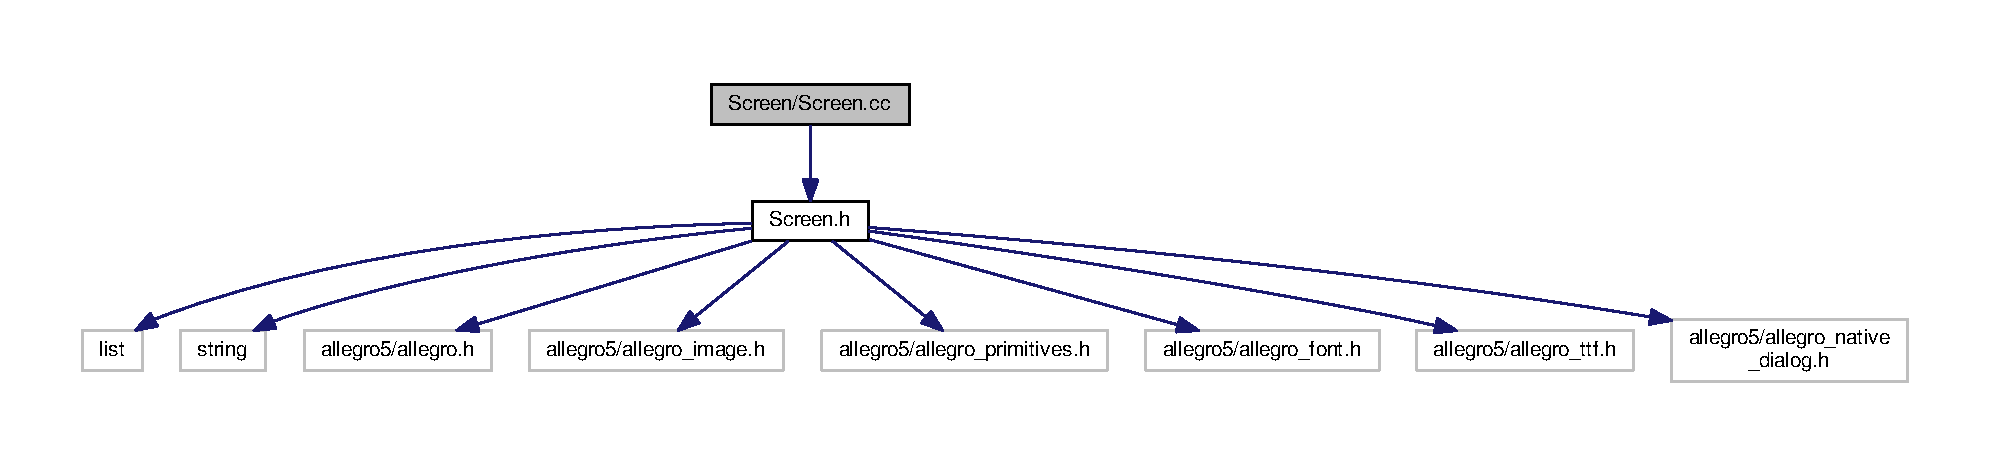
\includegraphics[width=350pt]{Screen_8cc__incl}
\end{center}
\end{figure}

\hypertarget{Screen_8h}{\section{Screen/\-Screen.h File Reference}
\label{Screen_8h}\index{Screen/\-Screen.\-h@{Screen/\-Screen.\-h}}
}
{\ttfamily \#include $<$list$>$}\\*
{\ttfamily \#include $<$string$>$}\\*
{\ttfamily \#include $<$allegro5/allegro.\-h$>$}\\*
{\ttfamily \#include $<$allegro5/allegro\-\_\-image.\-h$>$}\\*
{\ttfamily \#include $<$allegro5/allegro\-\_\-primitives.\-h$>$}\\*
{\ttfamily \#include $<$allegro5/allegro\-\_\-font.\-h$>$}\\*
{\ttfamily \#include $<$allegro5/allegro\-\_\-ttf.\-h$>$}\\*
{\ttfamily \#include $<$allegro5/allegro\-\_\-native\-\_\-dialog.\-h$>$}\\*
Include dependency graph for Screen.\-h\-:
\nopagebreak
\begin{figure}[H]
\begin{center}
\leavevmode
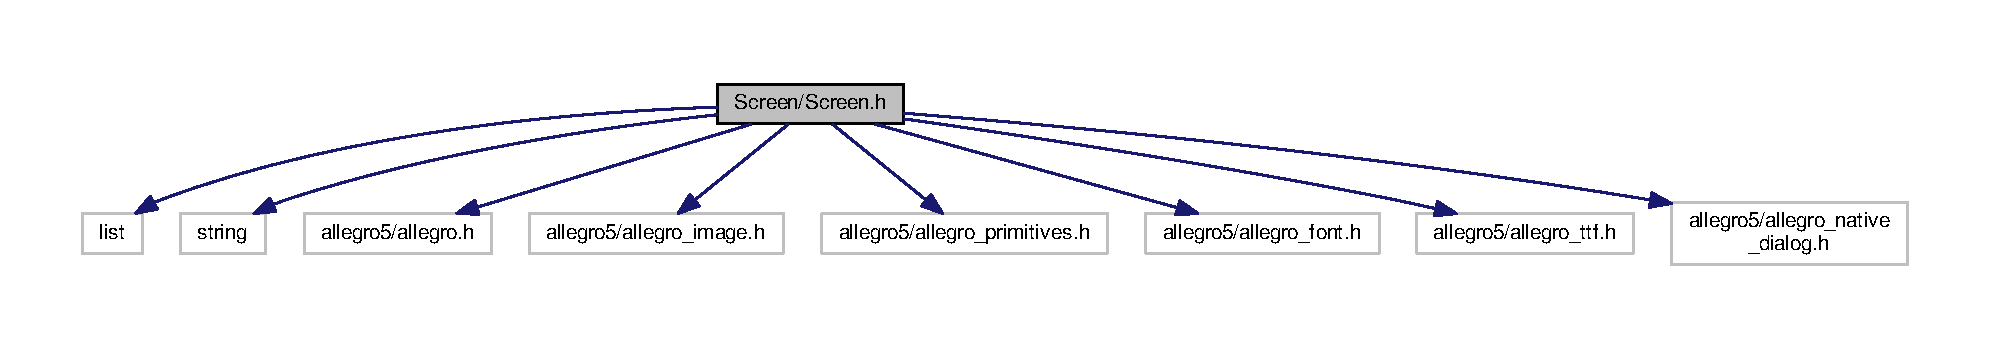
\includegraphics[width=350pt]{Screen_8h__incl}
\end{center}
\end{figure}
This graph shows which files directly or indirectly include this file\-:
\nopagebreak
\begin{figure}[H]
\begin{center}
\leavevmode
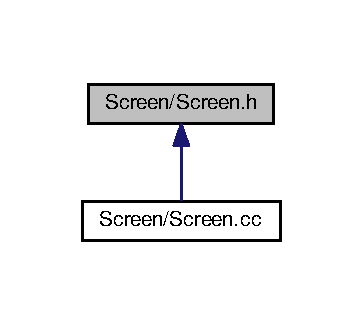
\includegraphics[width=174pt]{Screen_8h__dep__incl}
\end{center}
\end{figure}
\subsection*{Classes}
\begin{DoxyCompactItemize}
\item 
class \hyperlink{classMainScreen}{Main\-Screen}
\end{DoxyCompactItemize}

%--- End generated contents ---

% Index
\newpage
\phantomsection
\addcontentsline{toc}{part}{Index}
\printindex

\end{document}
